\PassOptionsToPackage{hypertexnames=false}{hyperref}
\documentclass[a4paper,fleqn]{cas-sc}
\usepackage[T1]{fontenc}
\usepackage{lmodern}
\usepackage[authoryear,round]{natbib}
\usepackage{amsmath,amssymb,amsthm}
\usepackage{booktabs}
\usepackage{array}
\usepackage{graphicx}
\usepackage{multirow}
\usepackage{float}
\usepackage{placeins}
\usepackage{needspace}
\renewcommand{\topfraction}{0.92}
\renewcommand{\floatpagefraction}{0.85}
\renewcommand{\textfraction}{0.07}
\setcounter{topnumber}{3}
\setcounter{totalnumber}{5}
\setlength{\textfloatsep}{16pt plus 4pt minus 2pt}
\setlength{\intextsep}{12pt plus 3pt minus 2pt}
\AtBeginDocument{%
  \setlength{\abovedisplayskip}{9pt plus 2pt minus 3pt}%
  \setlength{\belowdisplayskip}{9pt plus 2pt minus 3pt}%
}
\floatstyle{plaintop}
\newfloat{algo}{t}{loa}
\floatname{algo}{Algorithm}
\newtheorem{theorem}{Theorem}
\newtheorem{lemma}[theorem]{Lemma}
\newtheorem{proposition}[theorem]{Proposition}
\newtheorem{corollary}[theorem]{Corollary}
\newtheorem{example}[theorem]{Example}
\newtheorem*{uproposition}{Proposition}
\newdefinition{rmk}{Remark}
\newproof{pf}{Proof}
\newcommand{\R}{\mathbb{R}}
\newcommand{\E}{\mathbb{E}}
\newcommand{\norm}[1]{\lVert #1 \rVert}
\newcommand{\inner}[2]{\langle #1, #2 \rangle}
\newcommand{\odpair}{(s,t)}
\makeatletter
\AtBeginDocument{\gdef\lastpage{\@abspage@last}}
\makeatother
\ExplSyntaxOn
\RenewDocumentCommand \printorcid { }
  {
    \seq_if_empty:NF \g_stm_orcid_seq
      {
        \group_begin:
          \tex_let:D \thefootnote \relax \footnotetext
          {
            \raggedright
            \textsc{orcid}(s):\c_space_token
            \seq_use:Nn \g_stm_orcid_seq { ;~ }
          }
        \group_end:
      }
  }
\ExplSyntaxOff
\begin{document}
\hypersetup{bookmarksopen=true,bookmarksnumbered=true,
pdfkeywords={integrated gradients, traffic assignment, flow conservation, OD balance, cut consistency}}
\shorttitle{A Topological Theory of Spatial OD Attribution}
\shortauthors{Lei et al.}
\title[mode=title]{A Topological Theory of Spatial OD Attribution in Traffic Networks}
\author[1]{Da Lei}
\ead{dalei@scu.edu.cn}
\author[2]{Sylvia Y. He}
\cormark[1]
\ead{sylviahe@cuhk.edu.hk}
\author[3]{Shuli Luo}
\affiliation[1]{organization={Business School, Sichuan University},city={Chengdu},country={China}}
\affiliation[2]{organization={Department of Geography and Resource Management, The Chinese University of Hong Kong},city={New Territories},country={Hong Kong}}
\affiliation[3]{organization={School of Humanities and Social Science, The Chinese University of Hong Kong, Shenzhen},city={Shenzhen},country={China}}
\cortext[1]{Corresponding author: Sylvia Y. He.}
\begin{abstract}
The same origin--destination (OD) demand change can produce different cost
accounts at different traffic boundaries. We establish when these accounts
are interchangeable and how to compute and explain their differences on a
fixed road network. Necessary and sufficient conditions depend jointly on
network topology, the OD query, and the admissible region family. Arbitrary
separating regions constrain weights within every cycle atom, whereas regions
whose two sides are connected constrain only atoms on the queried block path;
off-path weights can remain heterogeneous. For general marginal costs, one
node-imbalance representation gives specified boundary accounts, exact
unrestricted extrema, the best common-value approximation, and maximum
boundary disagreement between models. A prefix scan also evaluates a
prescribed finite family of straight screenlines exactly. Same-state traffic
decompositions distinguish study and background responses under free-flow
and congestion weights. In Sioux Falls, positive system contributions coexist
with negative boundary accounts driven either by study congestion response
or by background congestion response. Anaheim extends the spatial calculation
and mechanism comparison to a larger network. An application to learned
assignment models evaluates spatial explanation errors alongside flow errors.
Together, the classification, computation and decomposition provide a
framework for interpreting spatial OD contributions.
\end{abstract}
\begin{keywords}
integrated gradients \sep traffic assignment \sep OD attribution \sep flow conservation \sep cut consistency
\end{keywords}
\maketitle
\hypersetup{pdfauthor={Da Lei, Sylvia Y. He, Shuli Luo}}
\section{Introduction}\label{sec:intro}
Transportation sensitivity analysis asks how changes in origin--destination
(OD) demand affect link flows and system outcomes
\citep{tobin1988sensitivity,josefsson2007sensitivity,patriksson2003aggregated}.
For a differentiable assignment model or learned surrogate, integrated
gradients allocate a finite outcome change across OD demands
\citep{sundararajan2017axiomatic}. Resolving this allocation through individual
link flows additionally locates the contribution on the network.

Consider a planner summarizing one demand change at several predetermined
corridor cross-sections or regional boundaries, using a fixed road partition.
The planner needs to know whether these summaries can replace one another;
if they differ, the task is to locate the intervening weighted response and
separate the queried traffic's adjustments from those of other traffic.
The inputs are the fixed network, demand change, outcome function and
candidate boundaries. The outputs are their OD accounts, an interchangeability
criterion, and an additive explanation of their differences.

The network-wide contribution $C_j$, attribution on roads within a region,
and signed boundary account $\phi_j(U)$ answer distinct questions.
Different boundaries define different outcome functions, so equality is a
structural property to establish rather than a prerequisite for attribution.
The proposed classification determines when the summaries share a common
boundary value across conservative responses. When they do not, a node
representation computes their differences and identifies the traffic
responses responsible. A negative boundary account can therefore be a
meaningful local cost response even when the network-wide OD contribution
is positive.

The question differs from tracking physical OD vehicles through screenlines
or cordons \citep{sheffi1985urban,vanzuylen1980most,bar2002origin}:
an OD-indexed sensitivity describes the network-wide response,
including other ODs' route changes, and weighting it by marginal
travel times or costs preserves additive completeness while creating
interior attribution sources and sinks --- on two series links, a
conservative unit response $(1,1)$ with weights $(w_1,w_2)$ balances
at the intermediate node only if $w_1=w_2$. Vehicle conservation
alone thus does not make outcome contributions interchangeable
across boundaries.

This distinction matters for explanations of conservative traffic
models: physical penalties, output projections, and exactly
conservative parameterizations constrain the predicted flows
\citep{raissi2019physics,shi2021physics,valente2025physics,richterpowell2022neural},
but conservation of those flows does not by itself make a learned
model's attribution interchangeable across boundaries. Exact
conservation transfers to flow-valued integrated gradients; outcome
weighting then imposes additional conditions on the network and the
outcome definition; and approximate output conservation may fail at
the first transfer step, because a small residual need not have small
OD derivatives.

The contribution has three connected parts. First, necessary and sufficient
topological conditions characterize boundary interchangeability for both
arbitrary separating regions and regions with two connected sides. The
region family changes the answer: only queried block paths constrain weights
in the latter case. Second, a common node representation computes selected
accounts, unrestricted extrema, approximate interchangeability and exact
model disagreement; a reusable geometric scan handles prescribed straight
screenlines. Third, same-state decompositions explain spatial differences
through study and background route responses under free-flow and congestion
weights. The cycle and block tools are classical; their coupling to the OD
query, region family and fixed attribution object is the central new result.
Endpoint identities and derivative-residual bounds support the calculation.
Learning comparisons demonstrate how the spatial framework evaluates
assignment explanations.

\section{Related work}\label{sec:related}
\paragraph{Attribution and cost allocation.}
Our edge-level object is input-specific conductance
\citep{dhamdhere2019important,lundstrom2022rigorous}: demand is the input,
link flow is an intermediate variable, and the traffic outcome is the output.
Its sum over links gives the integrated-gradient contribution of an OD.
Continuous marginal cost allocation also underlies Aumann--Shapley sharing
\citep{aumann1974values,billera1978internal}. Those scalar allocations and
computational-graph completeness do not impose node balance on a traffic
network. We analyze that additional property.

\paragraph{Conserved attribution flows on graphs.}
Graph-based explanation methods construct attribution flows with
boundary-consistency or conservation properties on directed acyclic
graphs: Shapley Flow makes edge attributions consistent across
different choices of explanatory boundary, with conservation at
internal nodes following from the efficiency axiom together with
boundary consistency, and the recursive
Shapley value recursively constructs edge-attribution flows that
conserve at internal nodes \citep{wang2021shapleyflow,singal2021rsv}.
Those works design
new attribution rules satisfying such axioms on computational or causal
graphs. Here the graph is a physical traffic network with cycles, the
edge-level conductance is fixed by the assignment model and outcome,
and the question is when these existing outcome-weighted sensitivities
have equal signed sums across OD-separating cuts, uniformly over
conservative responses, rather than when a newly constructed rule is
conserved.

\paragraph{Traffic models and sensitivity.}
Equilibrium sensitivity analysis studies demand-to-flow derivatives and their
aggregation \citep{tobin1988sensitivity,yang2005sensitivity,josefsson2007sensitivity,patriksson2003aggregated}.
Learned assignment maps, implicit optimization layers, and logit equilibrium
metamodels make such derivatives available to explanations
\citep{liu2023endtoend,amos2017optnet,lassen2025learning}.
Physical OD tracking through assignment and cordon counts concerns commodity
flows \citep{sheffi1985urban,vanzuylen1980most,bar2002origin}; it does not by
itself establish transferable budgets for marginal-cost-weighted attributions.

\paragraph{Conservation and graph structure.}
Physics-informed losses and conservative architectures constrain physical
outputs \citep{raissi2019physics,shi2021physics,richterpowell2022neural};
projections can enforce constraints exactly \citep{valente2025physics,baez2024guaranteeing}.
We examine their transfer to flow and outcome attributions; for
approximate conservation, derivative bounds of Landau--Kolmogorov type
are classical \citep{shadrin2014landau}, and
Appendix~\ref{app:approx} transfers such control to attribution
residuals. The relevant
circulation space and its decomposition into circuit classes are classical
\citep{oxley2011matroid,hopcroft1973algorithm}. The new classification couples
this decomposition to queried OD directions and their transitive equality
constraints.

\section{Attribution objects and balance criteria}\label{sec:objects}
\subsection{Edge attribution and the accounting question}
Let $\mathcal G=(V,E)$ be connected, with incidence matrix
$B\in\{-1,0,1\}^{n\times m}$ (negative at a link's tail), OD vectors
$\mu_j=e_{t_j}-e_{s_j}$, $s_j\ne t_j$, and $M=[\mu_1,\ldots,\mu_K]$.
Reciprocal and parallel arcs remain distinct edges when orientations are
forgotten. Let $f:\Omega\subset\R^K\to\R^m$ map demands to flows on an
open demand domain $\Omega$, and
$T:\R^m\to\R$ be a specified edgewise outcome. Assume both maps are $C^1$
on open neighborhoods of the relevant paths. With $\Delta q=q^1-q^0$ and
$\gamma(\lambda)=q^0+\lambda\Delta q$, define
\begin{align}
G_{:,j}&=\Delta q_j\int_0^1 J_f(\gamma(\lambda))\mathbf e_j\,d\lambda,
\label{eq:Gdef}\\
\widetilde C_{:,j}&=\Delta q_j\int_0^1 D_\lambda J_f(\gamma(\lambda))\mathbf e_j\,d\lambda,
\quad D_\lambda=\operatorname{diag}(\nabla T(f(\gamma(\lambda)))),
\label{eq:Cdef}\\
C_j&=\mathbf1^\top\widetilde C_{:,j},\qquad
\sum_j C_j=T(f(q^1))-T(f(q^0)).\label{eq:Cscalar}
\end{align}
$G$ attributes flow changes; $\widetilde C$ resolves the outcome contribution
through links; $C_j$ is its scalar OD contribution. Their columns are signed
system sensitivities, including other ODs' route adjustments, rather than
physical commodity flows. Entry $\widetilde C_{e,j}$ is input-specific
conductance through link $e$ \citep{dhamdhere2019important}.\label{sec:whyC}

If $Bf(q)=Mq$, differentiation and integration give
\begin{equation}
BJ_f(q)=M,\qquad BG_{:,j}=\mu_j\Delta q_j.\label{eq:anchorchain}
\end{equation}
The same conclusion holds for $Bf(q)=Mq+b$ with constant background demand
balance $b$. Outcome attribution is \emph{same-OD balanced} when
$B\widetilde C_{:,j}=\beta_j\mu_j$ for some $\beta_j\in\R$.
The scale $\beta_j$ is a boundary value, generally different from $C_j$:
on two series links with unit weights, $C_j=2\Delta q_j$ but
$\beta_j=\Delta q_j$.

For $s_j\in U\subseteq V\setminus\{t_j\}$, orient the cut account as
$\phi_j(U)=-\mathbf1_U^\top B\widetilde C_{:,j}$, and write
$b_j=B\widetilde C_{:,j}$. Any two separating sets satisfy
\begin{equation}
\phi_j(U')-\phi_j(U)
=-\sum_{v\in U'\setminus U}b_{jv}
+\sum_{v\in U\setminus U'}b_{jv};
\label{eq:cutdiff}
\end{equation}
for nested sets $U\subseteq U'$ the second term vanishes, leaving
$\phi_j(U')-\phi_j(U)=-\sum_{v\in U'\setminus U}(B\widetilde C_{:,j})_v$.
The difference between two boundaries is thus the enclosed imbalance,
with incoming and outgoing regions entering with opposite signs.
For a separable outcome $T(F)=\sum_e g_e(F_e)$, the account itself
also has a direct reading. With $\delta^+(U)$ and $\delta^-(U)$ the
arcs leaving and entering $U$,
\begin{equation}
H_U(F)=\sum_{e\in\delta^+(U)}g_e(F_e)-\sum_{e\in\delta^-(U)}g_e(F_e),
\qquad
\phi_j(U)=\operatorname{IG}_j[\,H_U\circ f\,],
\label{eq:hboundary}
\end{equation}
because each entry $\widetilde C_{e,j}$ of Eq.~\eqref{eq:Cdef} is the
integrated gradient of the scalar outcome $g_e\circ f$, and the
incidence signs turn $-\mathbf 1_U^\top B\widetilde C_{:,j}$ into the
signed boundary sum of $H_U$. For TSTT, $\phi_j(U)$ therefore
attributes the demand change to the excess of the total travel cost on
the region's outgoing arcs over that on its incoming arcs: a
boundary-related outcome in its own right, neither the region's
internal cost nor a vehicle count.
\begin{uproposition}[cut-consistency equivalence]\label{par:cutequiv}
Same-OD balance holds exactly when every separating cut has one common
signed value $\phi_j(U)=\beta_j$.
\end{uproposition}
Indeed, balance implies this identity. Conversely, comparing $\{s_j\}$
with $\{s_j,v\}$ forces zero divergence at every interior node; the two
endpoint entries are then opposite because incidence columns sum to zero.

\begin{table}[pos=tb]
\caption{Three spatial summaries of one OD attribution. $E_R$ is a road set
specified before aggregation.}\label{tab:objects}
\begin{tabular*}{\tblwidth}{@{}p{5cm}p{9cm}@{}}
\toprule Object & Transportation question\\\midrule
$C_j=\sum_e\widetilde C_{e,j}$ & How much does this OD contribute to the system outcome change?\\
$\sum_{e\in E_R}\widetilde C_{e,j}$ & How much of that contribution is located on the specified regional roads?\\
$\phi_j(U)$ & What is its signed aggregation on the specified boundary?\\
\bottomrule\end{tabular*}\end{table}

Throughout, $\mathcal U_j^{\mathrm{all}}$ contains all sets separating
$s_j$ from $t_j$; $\mathcal U_j^{\mathrm{conn}}$ restricts both induced sides
to be connected in the underlying undirected network; and
$\mathcal U_j^{\mathrm{geo}}$ is a specified finite family of straight
screenline regions, filtered for two-sided connectivity.
The unrestricted extrema below are closed-form exact values. Sioux Falls
connected extrema use complete enumeration. Geometric extrema and Anaheim's
selected connected-region ranges are exact only over their stated finite
families, and do not determine extrema over all connected regions.

\subsection{Pointwise guarantees and realized balance}\label{sec:levels}\label{sec:hierarchy}
At fixed weights $D=\operatorname{diag}(w)$, realized-model balance
requires $BDJ_j=\alpha_j\mu_j$ for the model's actual response.
Universal directional balance requires $BDx\in\operatorname{span}\{\mu_j\}$
for every $Bx=\mu_j$, allowing its coefficient to depend on $x$.
\emph{Structural compatibility} additionally requires one common coefficient
across all such responses. The last property is what we classify.
For non-collinear queries with shared weights, universal directional
balance already implies structural compatibility because
$BD\ker B\subseteq\bigcap_j\operatorname{span}\{\mu_j\}=\{0\}$;
a query and its reverse alone do not suffice.
Pointwise balance along the demand path implies integrated balance;
the converse can fail through cancellation. Appendix~\ref{supp:criteria}
gives examples and restricted-response results. Thus a realized attribution
can balance without satisfying the universal structural conditions.

\section{Topology, OD queries and admissible regions}\label{sec:classification}
Take the block-cut tree of the underlying undirected multigraph.
Its non-bridge blocks, together with each bridge as a singleton,
are the \emph{cycle atoms}. They are the classical graphic-matroid circuit
classes, with each bridge retained separately. The \emph{OD block path}
$\mathcal P(s,t)$ is the atom sequence on the unique block-cut-tree path
between the OD endpoints. For several queries, merge all atoms traversed
by each $\mathcal P_j=\mathcal P(s_j,t_j)$ and take the transitive closure.
The resulting edge sets $\bar E_1,\ldots,\bar E_{K'}$ are the
\emph{OD-compatibility classes}; atoms on no queried path remain separate.

\Needspace{15\baselineskip}
\begin{theorem}[single-OD classification, static form]\label{thm:t3cpmain}
Let $\mathcal{G}$ be a connected multigraph with one OD pair $(s,t)$,
\textbf{$s\neq t$}, let
$w\in\R^m$, and let $D=\operatorname{diag}(w)$. The
\emph{response-independent same-OD balance property}
\begin{equation}
\exists\,\alpha\in\R:\qquad BDx=\alpha\,\mu
\quad\text{for every }x\in\R^m\text{ with }Bx=\mu,
\label{eq:t3prop}
\end{equation}
with the scale $\alpha$ independent of the response $x$, holds
\textbf{if and only if}
\begin{enumerate}[(i)]
\item $w$ is constant within every non-bridge atom; and
\item all atoms on the $s$--$t$ block path $\mathcal{P}(s,t)$ share
one common value.
\end{enumerate}
In that case every conservative response induces the same boundary vector:
$BDx=w^*\mu$ for every $x$ with $Bx=\mu$, where
$w^*:=w|_{\bigcup\mathcal{P}(s,t)}$ is the common value of (ii) and
$\alpha=w^*$ is the scale in \eqref{eq:t3prop}.
\end{theorem}

Condition (i) concerns every atom, including those off the OD path. Their
constants may differ; only the traversed atoms must share the scale $w^*$.
The proof adds a virtual edge from $t$ back to $s$
(Appendix~\ref{app:classificationproof}): conservative OD responses then
become circulations on the extended graph, so the boundary vector is
response-independent exactly when diagonal weighting preserves the
circulation space --- equivalently, when every weighted cycle has zero
node divergence --- which forces equal weights within each cycle atom
and one shared weight along the atoms the OD block path connects.
\begin{figure}[pos=t]
\centering
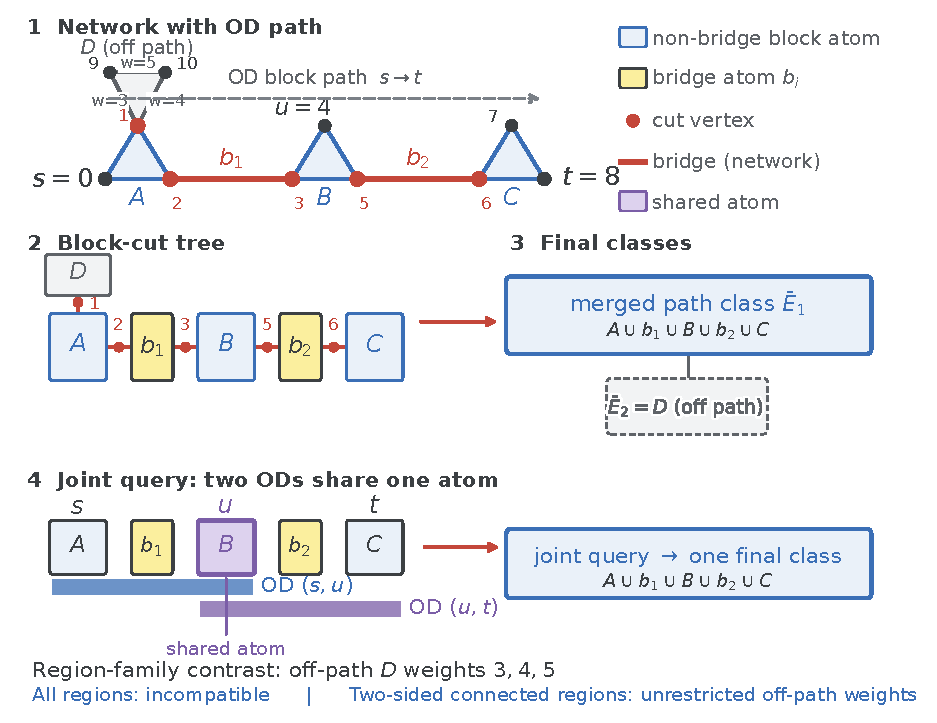
\includegraphics[width=0.90\linewidth]{../figures/fig2_block_cut_v103.pdf}
\caption{OD queries merge the atoms they traverse. Two paths sharing atom
$B$ merge the full chain transitively; off-path atom $D$ stays separate.
For the connected-region comparison, atom $D$ has heterogeneous weights
$3,4,5$: these are invisible to the queried connected boundaries, but
violate unrestricted interchangeability. Orientations are omitted; node
numbering starts at zero.}
\label{fig:blockcut}
\end{figure}

\begin{theorem}[multi-OD classification, static form at a shared
realized flow state]\label{thm:t3cm}
Let $\mathcal{G}$ be connected, let each OD pair satisfy $s_j\neq t_j$,
and let $w\in\R^m$, $D=\operatorname{diag}(w)$. The
response-independent same-OD balance property \eqref{eq:t3prop}
--- for each queried $j$, some $\alpha_j\in\R$ with
$BDx=\alpha_j\mu_j$ for every $x$ with $Bx=\mu_j$ --- holds
simultaneously for the queried ODs \textbf{if and only if} $w$ is
constant on each OD-compatibility class $\bar{E}_k$.
\end{theorem}

The classification concerns all signed responses compatible with vehicle
conservation; an equilibrium model generally realizes only a subset of
these responses (Appendix~\ref{app:membership}).
All queries use the same realized weight vector. Queries with $\Delta q_j=0$
have zero attribution columns and need not enter the closure. Requiring all
ordered pairs of distinct vertices collapses the classes to one per
connected component (Corollary~\ref{cor:allod}).


\begin{corollary}[path form: endpoint implication]\label{cor:path}
Let $f\in C^1$ be conservative on an open set, $T\in C^1$,
$\gamma(\lambda)=q^0+\lambda\Delta q$ the straight-line path with $\Delta q\ne0$, and
$w(\lambda)=\nabla T(f(\gamma(\lambda)))$, $D_\lambda=\operatorname{diag}(w(\lambda))$, shared by
all participating ODs. If the equivalent conditions of
Theorems~\ref{thm:t3cpmain} and~\ref{thm:t3cm} hold at $w(\lambda)$ for
every $\lambda\in[0,1]$, then, for every participating $j$
simultaneously, the endpoint balance
\[
B\widetilde{C}_{:,j}=\beta_j\,\mu_j
\]
holds with
\[
\beta_j=\Delta q_j\int_0^1 w^*_{k(j)}(\lambda)\,d\lambda,
\]
where $w^*_{k(j)}$
is the common value on the compatibility class $k(j)$ containing the
atoms of $\mathcal{P}_j$.
\end{corollary}

Figure~\ref{fig:blockcut} becomes a constructive design example in
Table~\ref{tab:topologyexample}. We use its $11$-node, $14$-edge graph
with $s=0$, $u=4$, $t=8$ and the linear structural outcome $T_w(F)=w^\top F$.
Initially the query $(s,u)$ joins $A,b_1,B$, while $b_2$, $C$, and
$D$ can retain their own constants. Adding $(u,t)$ joins the remaining
chain through their shared atom $B$. Adjusting only $b_2$ and $C$
then restores a common account for both queries while retaining the
unrelated atom's weight $3$.
\begin{table}[pos=tb]
\caption{Constructive query-dependent compatibility on Figure~\ref{fig:blockcut}.
Ranges use all $512$ separating sets per query and a conservative unit response;
the weighted circulation residual is below $5\times10^{-16}$ in all stages,
so these ranges are independent of that response.}\label{tab:topologyexample}
\begin{tabular*}{\tblwidth}{@{\extracolsep{\fill}}lccccl}
\toprule Stage & $w_{A,b_1,B}$ & $w_{b_2,C}$ & $w_D$ & Queried ODs & Account ranges\\\midrule
Initial query & 1 & 2 & 3 & $(s,u)$ & $[1,1]$\\
Add query & 1 & 2 & 3 & $(s,u);(u,t)$ & $[1,1];[1,2]$\\
Adjust merged class & 1 & 1 & 3 & $(s,u);(u,t)$ & $[1,1];[1,1]$\\
\bottomrule\end{tabular*}\end{table}
The calculation uses the minimum-norm solution of $Bx=\mu$ and checks
$BDZ=0$ on a basis of $\ker B$, which establishes response independence
of the displayed boundary vector. The theorem supplies the uniform
common-account guarantee in stages one and three. These intentionally
chosen linear weights illustrate compatibility; they are not asserted
to be the marginal costs of the original TSTT outcome.

Off-path atoms are constrained here because a signed circulation can
be added to any conservative response, and heterogeneous weights can turn
it into node divergence. Connected regions change this conclusion.

\subsection{Compatibility for connected traffic regions}\label{sec:connectedclassification}
The admissible region family changes the structural answer. Let
\[
\mathcal U^{\mathrm{conn}}_{st}=\{U\subset V:s\in U,\ t\notin U,
\ G[U]\text{ and }G[V\setminus U]\text{ are connected}\},
\]
where connectivity uses the underlying undirected multigraph. These are
separating bonds: both sides of the boundary form connected regions.
\begin{theorem}[two-sided connected-region classification]\label{thm:connectedclassification}
For a connected loopless multigraph, $\mu=e_t-e_s$, and
$D=\operatorname{diag}(w)$, the property
\begin{equation}
\exists\alpha\in\R\quad\forall x\text{ with }Bx=\mu\quad
\forall U\in\mathcal U^{\mathrm{conn}}_{st}:
-\mathbf1_U^\top BDx=\alpha
\label{eq:connectedclassification}
\end{equation}
holds if and only if every edge in the atoms of $\mathcal P(s,t)$ has
one common weight $\alpha$. Weights of edges outside those atoms are
arbitrary, even within an off-path cycle atom.
\end{theorem}
The proof in Appendix~\ref{app:connectedproof} uses connected prefix and
suffix regions within each traversed atom. Each admissible boundary
crosses edges in just one such atom, which explains why off-path
heterogeneity is invisible to this region family. This is a universal
fixed-weight statement; agreement for one realized response need not
imply its conditions.

\begin{corollary}[several queries on connected regions]\label{cor:connectedmulti}
At one shared weight vector, Eq.~\eqref{eq:connectedclassification} holds
for all queried ODs if and only if edges in each group of atoms joined
by the queried block paths have one common weight. An atom on no queried
path has no weight restriction, including no within-atom restriction.
\end{corollary}
Thus restricting attention to connected traffic regions permits additional
outcome heterogeneity. It changes the compatibility classification,
while the unrestricted extrema and error formulas below retain their
own stated boundary family.

\paragraph{A constructive distinction on Figure~\ref{fig:blockcut}.}
Keep weights $1$ on $A,b_1,B$, weights $2$ on $b_2,C$, but set the three
off-path $D$ weights to $3,4,5$. The first query $(s,u)$ admits common
account $1$ on every two-sided connected region for every conservative
response. The second query $(u,t)$ initially has connected accounts
spanning $[1,2]$ and fails that criterion. Changing only $b_2,C$ to
weight $1$ makes both queries compatible on connected regions, while
$D$ remains internally heterogeneous. For each query there are $512$
unrestricted separating sets but only $5$ two-sided connected sets.
Checking a particular response and a complete circulation basis confirms
the universal connected-region assertions; this is stronger than checking
sampled responses. A unit signed circulation in $D$ gives unrestricted
accounts $[-1,3]$ after the merge, while all connected accounts remain
$1$. Thus the unrestricted criterion still fails. This fixed structural
outcome illustrates the theorem; its weights do not replace the original
TSTT marginal costs. The reproducible record is provided with the code.


\subsection{Linear outcomes and transportation costs}\label{sec:transport}
\begin{corollary}[linear outcome functionals]\label{cor:linear}
Let $f\in C^1$ be exactly conservative on an open neighborhood of the
attribution path, and let $T(F)=a^\top F$ be a linear functional of
realized flows. Then $\nabla T\equiv a$, so response-independent
cut balance holds if and
only if $a$ is constant on the compatibility classes --- a
condition on the outcome definition alone, checkable by
inspection before any model is trained. The pointwise classification
then holds at every $\lambda$, with common cut account
$\beta_j=\Delta q_j\,a|_{\bigcup\mathcal{P}_j}$ exactly.
\end{corollary}

Nonlinear compatible outcomes also exist: if
$T(F)=\Phi(\sum_{e\in\bar E_1}F_e,\ldots,\sum_{e\in\bar E_{K'}}F_e)$,
its gradient is class-constant at every flow. More familiar traffic outcomes
require equality of their actual marginal weights. The Beckmann potential
has weights $t_e(F_e)$; total system travel time (TSTT) has weights
$t_e(F_e)+F_et'_e(F_e)$; a separable index $\sum_e g_e(F_e)$ has
weights $g'_e(F_e)$. Heterogeneous link parameters and congestion typically
violate these equalities. A single-link outcome has a nonzero common boundary value
only when the queried OD block path is precisely that singleton bridge.

\subsection{Endpoint cancellation and network representation}\label{sec:cancellation}
On two series links, an outcome whose marginal weights oscillate around
unity can integrate to the same balanced column $(1,1)$ as the linear
outcome on one demand segment, yet fail to balance on another; the
linear outcome gives the same composite demand-to-outcome map with
balanced edge attributions on every segment
(Example~\ref{ex:cancellation}). The specified edgewise outcome
therefore matters even at fixed network topology.

The network representation matters as well: subdividing a link leaves
the composite map unchanged but creates interior divergence
$\tau(2\alpha-1)\Delta q$, and even the balanced split $\alpha=1/2$
halves the original cut value (Example~\ref{ex:subdivision}).
Response independence concerns conservative responses on a fixed network;
it does not make the account invariant to road subdivision.

\section{Exact spatial computation}\label{sec:stability}\label{sec:algorithm}
Once the classes are constructed, structural compatibility is tested by
\[
\eta(\lambda)=\max_k\max_{e\in\bar E_k}|w_e(\lambda)-\bar w_k(\lambda)|,
\qquad
\bar w_k=|\bar E_k|^{-1}\sum_{e\in\bar E_k}w_e.
\]
The joint condition is exactly $\eta=0$. Class construction uses the
block-cut tree and transitive merging; testing a weight vector then needs
one edge scan. No fitted-model derivatives are required for a linear outcome.

For a realized integrated attribution, define
\begin{equation}
d_j=(I-P_{\mu_j})B\widetilde C_{:,j},\qquad
P_{\mu_j}=\frac{\mu_j\mu_j^\top}{\norm{\mu_j}_2^2}.
\label{eq:endpointd}
\end{equation}
Endpoint cut consistency holds precisely when $d_j=0$; only then does
$\mu_j^\top B\widetilde C_{:,j}/\norm{\mu_j}_2^2$ represent a common cut
value, whatever mechanism produced the balance
(Section~\ref{sec:levels}).

Without a connectivity restriction, each interior node can enter the
separating set independently. Therefore Eq.~\eqref{eq:cutdiff} gives
\begin{equation}
S_j:=\max_U\phi_j(U)-\min_U\phi_j(U)
=\sum_{v\notin\{s_j,t_j\}}|(B\widetilde C_{:,j})_v|.
\label{eq:cutspread}
\end{equation}
The extrema themselves have a closed form: writing $b_j=B\widetilde
C_{:,j}$, $(x)_+=\max(x,0)$, and summing over interior nodes
$v\notin\{s_j,t_j\}$,
\begin{equation}
\phi_j^{\min}=\phi_j(\{s_j\})-\sum_v(b_{jv})_+,
\qquad
\phi_j^{\max}=\phi_j(\{s_j\})+\sum_v(-b_{jv})_+,
\label{eq:cutextrema}
\end{equation}
since the minimizing set retains exactly the interior nodes with
positive divergence. Subtracting gives, for every separating set $U$
with $I_j=V\setminus\{s_j,t_j\}$,
\begin{equation}
\phi_j(U)-\phi_j^{\min}
=\sum_{v\in I_j\setminus U}(b_{jv})_+
+\sum_{v\in I_j\cap U}(-b_{jv})_+,
\label{eq:cutgap}
\end{equation}
so the gap to the unrestricted minimum is exactly the positive
divergence the region omits plus the negative divergence it contains.
When $\phi_j(\{s_j\})>0$, the unrestricted family
therefore contains a negative account whenever the interior positive
divergence $\sum_v(b_{jv})_+$ exceeds the origin-cut account: node
imbalance, extremal location, and sign crossing are the same statement.
$S_j=0$ is equivalent to $d_j=0$.
The projector in Eq.~\eqref{eq:endpointd} changes only the two endpoint
entries. Cauchy--Schwarz on the $n-2$ interior entries therefore gives
\begin{equation}
S_j=\sum_{v\notin\{s_j,t_j\}}|(d_j)_v|
\le\sqrt{n-2}\,\norm{d_j}_2.
\label{eq:rangebound}
\end{equation}
For network regions whose induced subgraphs and complements are both
connected, define $S_j^{\mathrm{conn}}$ by restricting the same extrema to
that family. Then $S_j^{\mathrm{conn}}\le S_j$; a small restricted range
alone does not establish the full structural criterion. We report both
ranges as percentages of the absolute origin-cut value
$|\phi_j(\{s_j\})|$, which remains explicit because the ratio depends
on that denominator (absolute ranges when it is zero).

\begin{corollary}[best common boundary value]\label{cor:approxinterchange}
For the unrestricted family, the unique best constant in maximum absolute
account error is
\[
\beta_j^\star=\frac{\phi_j^{\max}+\phi_j^{\min}}2
=\frac{(b_j)_{t_j}-(b_j)_{s_j}}2,\qquad
\min_{\beta\in\mathbb R}\max_{U\in\mathcal U_j^{\mathrm{all}}}
|\phi_j(U)-\beta|=\frac{S_j}{2}.
\]
Hence all separating accounts lie within a prescribed absolute tolerance
$\varepsilon$ of some common value if and only if $S_j\le2\varepsilon$.
\end{corollary}
\begin{proof}
For any constant, its largest error at the two attained extrema is at least
half their difference; their midpoint attains this bound for every account.
Equation~\eqref{eq:cutextrema} and $\mathbf1^\top b_j=0$ give the midpoint formula.
\end{proof}
The coefficient agrees with the endpoint projection in
Eq.~\eqref{eq:endpointd}. It approximates the original accounts; it does
not change their edge attribution or define a new system contribution.

\subsection{Exact boundary error and response supervision}\label{sec:boundarylearning}
For a query $j$ and any edge vector $h$, define the seminorm
\begin{equation}
\mathcal K_j(h)=\frac12\left(\left|(Bh)_{t_j}-(Bh)_{s_j}\right|
+\sum_{v\notin\{s_j,t_j\}}|(Bh)_v|\right).
\label{eq:boundaryseminorm}
\end{equation}
\begin{corollary}[exact maximum boundary error]\label{cor:boundaryerror}
Let $e_j=\widetilde C^L_{:,j}-\widetilde C^S_{:,j}$ be the difference
between learned and reference attribution columns. Then
\begin{equation}
\max_{U:s_j\in U,\ t_j\notin U}|\phi_j^L(U)-\phi_j^S(U)|
=\mathcal K_j(e_j).\label{eq:exactboundaryerror}
\end{equation}
At a common demand $q$, write
$h_j(q)=D^L(q)J_j^L(q)-D^S(q)J_j^S(q)$.
For any subfamily $\mathcal U_j$ of separating boundaries,
\begin{equation}
\epsilon_j^{\mathcal U}:=\max_{U\in\mathcal U_j}|\phi_j^L(U)-\phi_j^S(U)|
\le |\Delta q_j|\int_0^1\mathcal K_j(h_j(\gamma(\lambda)))\,d\lambda.
\label{eq:localboundarybound}
\end{equation}
\end{corollary}
The proof in Appendix~\ref{app:boundaryerror} applies
Eq.~\eqref{eq:cutextrema} to the error column. Evaluation requires one
incidence multiplication and node scan, without enumerating boundaries.
Connected regions and straight screenlines inherit an upper bound; their
restricted maxima need not equal $\mathcal K_j(e_j)$. The endpoint term
must be retained: the two explanations may each be cut-consistent but
have different common boundary values, which internal imbalance alone misses.

The seminorm evaluates spatial explanation errors directly. It also defines
reference-matching losses, whose complete specifications are collected in
Appendix~\ref{app:learning-objectives}. Their comparison is an application
of the spatial framework (Section~\ref{sec:pairresults}).

\begin{algo}[t]
\caption{Spatial accounts from an attribution column}\label{alg:spatial}
\small
\textbf{Input:} incidence $B$, query $(s_j,t_j)$, edge attribution $c_j$,
selected regions $U,W$, and optionally a comparison column $c'_j$.\\
1. Compute $b_j=Bc_j$; return its node distribution.\\
2. Return $\phi_j(U)=-\mathbf1_U^\top b_j$ and
$\phi_j(U)-\phi_j(W)=-(\mathbf1_U-\mathbf1_W)^\top b_j$.\\
3. Scan interior nodes to return the extrema in Eq.~\eqref{eq:cutextrema}
and their sets $\{s_j\}\cup\{v:b_{jv}>0\}$ and
$\{s_j\}\cup\{v:b_{jv}<0\}$.\\
4. If $c'_j$ is supplied, return $\mathcal K_j(c_j-c'_j)$ as the exact
maximum absolute error over unrestricted separating regions.\\
The incidence product and scan cost $O(|E|+|V|)$ per column; selected-region
sums cost $O(|V|)$. The same node representation serves all these tasks. The columns must already
have been computed; their reference-attribution cost remains separate.
\end{algo}

\subsection{Exact scanning of predefined straight screenlines}\label{sec:scan}
Fix $D$ directions before evaluating attribution. For each direction, sort nodes by their coordinate projection and group equal projection values; no screenline splits such a group. A candidate position is a gap between adjacent groups. Forward and reverse union--find sweeps record whether each prefix and suffix induces a connected subgraph. This geometry and topology preprocessing is reusable across queries, demand paths and models.
For one attribution column, form $b_j=B\widetilde C_{:,j}$ and prefix sums $P_{j,k}=\sum_{i\leq k}(b_j)_{\pi(i)}$. If $s_j$ lies in the prefix and $t_j$ outside, its account is $-P_{j,k}$; for the reverse orientation it is $P_{j,k}$ because $\mathbf1^\top b_j=0$. Retain only endpoint-separating gaps with both sides connected. Scanning these values gives exact accounts and extrema over this prescribed finite screenline family. It does not optimize over every possible direction in the plane. Preprocessing takes $O(D(|V|\log|V|+|E|\alpha(|V|)))$; after preprocessing, a column takes $O(|E|+D|V|)$ using sparse incidence multiplication. Duplicate regions may be removed without changing extrema.

On Sioux Falls, 36 directions at five-degree intervals give 1642 admissible query--position accounts across six queries (duplicates across directions retained for both algorithms). Direct summation recomputes outgoing minus incoming crossing-edge contributions on exactly these same oriented regions. The largest account discrepancy was 2.2e-11 TSTT units. Reusable preprocessing took 83.48 ms. \begin{table}[t]\centering\small\caption{Same-task spatial aggregation after reference columns are available. Median batch times; reference generation is excluded. The 120-column workload repeats the six columns twenty times and measures repeated-query cost, not additional empirical evidence.}\label{tab:scan}\begin{tabular}{rrrr}\toprule Columns & Accounts & Prefix scan (ms) & Direct crossings (ms)\\\midrule
6 & 1642 & 4.16 & 28.51\\
120 & 32840 & 87.92 & 1176.15\\
\bottomrule\end{tabular}\end{table}


\paragraph{Scope and approximate conservation.}\label{sec:noninheritance}
The classification fixes the road representation, outcome weights and
admissible regions, and quantifies over all signed conservative responses.
For a model with residual $r(q)=Bf(q)-Mq-b$ and constant $b$, the corresponding
flow-attribution residual is
\begin{equation}
R_j:=BG_{:,j}-\mu_j\Delta q_j
=\Delta q_j\int_0^1\partial_jr(\gamma(\lambda))\,d\lambda,
\qquad \sum_jR_j=r(q^1)-r(q^0).
\label{eq:residualidentity}
\end{equation}
Small endpoint residuals control the sum, but individual columns can cancel.
Appendix~\ref{app:approx} gives derivative-regularity conditions, a local
bound, sharpness examples and an extension to weighted accounts. The traffic
experiments below use exactly conservative models.

\section{Numerical evidence and transportation interpretation}\label{sec:numerics}
For Sioux Falls, all reported absolute TSTT accounts use benchmark flows in veh/h and time
units of $0.01$ h; multiply a reported number by $0.01$ to obtain the
hourly vehicle-hour total. This convention applies to the Sioux Falls attribution and error tables.
Anaheim instead uses minutes, as specified separately in Section~\ref{sec:anaheim}.
\subsection{Study design and local mechanism}
The Sioux Falls experiment compares an exactly conservative learned surrogate
with direct fixed-path logit-SUE on eight OD queries. The two evidence
types divide the labour: Figure~\ref{fig:blockcut} illustrates the
classification's query dependence on a network whose queries merge atoms
differently, whereas here all $76$ arcs lie in one compatibility class,
the structural weight condition is the same for every OD, and the
experiment instead measures what boundary differences heterogeneous
realized cost weights produce under equilibrium responses. The OD
differences reported below thus arise from realized responses, weight
dispersion, and integration, not from different compatibility classes.
Each study OD uses ten
fixed paths. We compare zero background (A), frozen background flows (B),
and joint re-equilibration at fixed background demands (C). Setting C loads
all $528$ positive-demand OD pairs but attributes changes only to the eight
study demands, selected as the eight largest published demands --- all
involving node $10$, a local rather than representative comparison.
Appendix~\ref{supp:fields} gives the full settings.

Each study demand moves from $0.2q_{\mathrm{base}}$ to $1.6q_{\mathrm{base}}$
along a straight line ($q_{\mathrm{base}}$: the eight published
demands, $3{,}900$--$4{,}400$ veh/h); the eight-query experiments use this demand
segment unless otherwise stated. The three settings differ only in how
the remaining demands are handled.

The settings also differ in the redistribution directions their
fixed path sets can express: setting A's path-exchange space
$T_{\mathrm{swap}}$ (Appendix~\ref{app:membership}) has dimension
$32$, a proper subspace of the $53$-dimensional circulation space,
while setting C's full-background path set spans the complete space
($53=m-n+1$; Appendix~\ref{supp:networks}). Spanning the circulation
space is a statement about linear directions, not about which signed
responses the logit-SUE Jacobian realizes.

Uniform weights are a compatible control. The inactive-link outcome
$T(F)=F_{1\to2}$ gives zero attribution because that arc lies outside
the setting-A surrogate path union (setting C's path sets cover every
arc). The active-link outcome $T(F)=F_{10\to16}$ gives
$BDx=\mu_{(10,16)}x_{10\to16}$: direction is preserved for that OD, while
circulations can change the scale. TSTT instead weights the response by
heterogeneous marginal social costs and produces interior node imbalance.
Figure~\ref{fig:respfield} shows these three patterns on the same realized
learned response.
\begin{figure}[htbp]
\centering
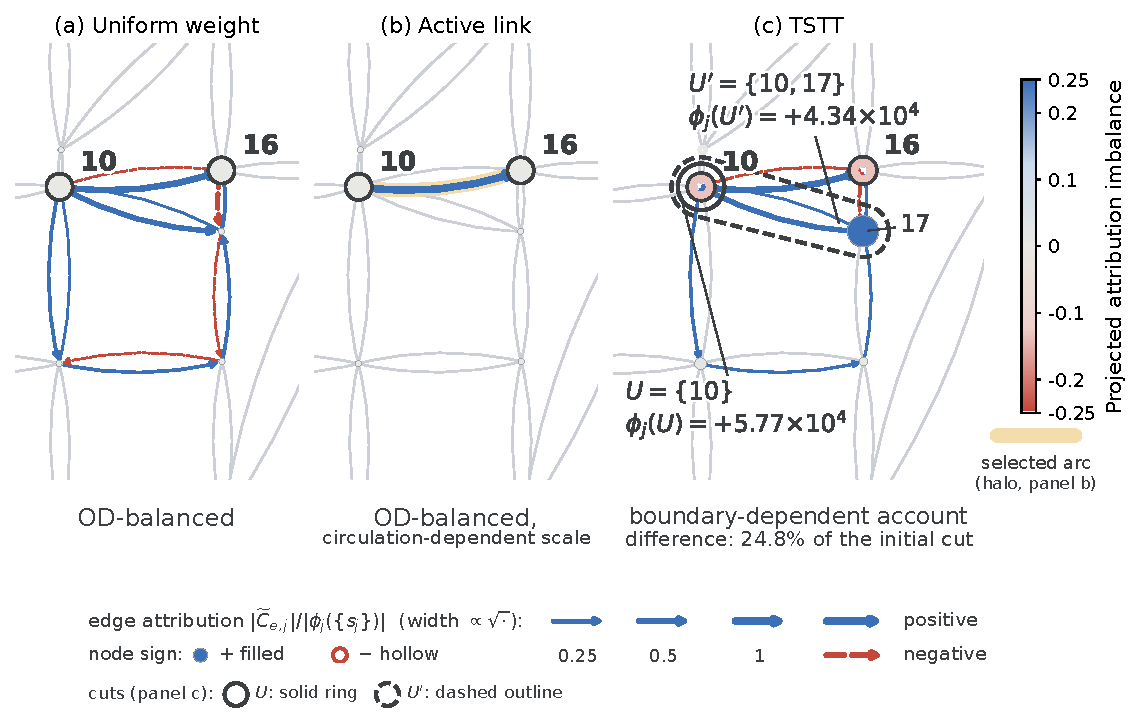
\includegraphics[width=0.84\linewidth]{../figures/fig_resp_field_v100.pdf}
\caption{OD $(10,16)$ endpoint attributions, zero background, learned
seed $0$. (a) Uniform weights give cut consistency. (b) The active-link
outcome balances in the OD direction but has no response-independent scale.
(c) The signed TSTT boundary account decreases by $24.8\%$ when the
boundary expands from $\{10\}$ to $\{10,17\}$.
Widths encode attribution magnitude; node colors show the projected
attribution imbalance $(d_j)_v$ (Eq.~\eqref{eq:endpointd}) divided by
the absolute origin-cut value.}
\label{fig:respfield}
\end{figure}
For the seed-$0$ TSTT account, adding node $17$ to $U=\{10\}$ lowers
$\phi_j(U)$ from $5.77\times10^4$ to $4.34\times10^4$ --- the largest
of the $22$ single-node enlargements, accounting for about $92\%$ of
the unrestricted range, with the direct-SUE counterpart at $24.80\%$
(Section~\ref{subsec:bgsplit}); both displayed regions and their
complements are network-connected.
The free-flow component contributes $84.7\%$ of the node-$17$ imbalance,
the congestion premium $15.3\%$; the ordering reverses at the negative
minima of Section~\ref{subsec:newod}, where the congestion premium
dominates (Table~\ref{tab:ffcong}). All incident links have free-flow time
$2$ except $10\leftrightarrow17$, which has time $8$; exact vehicle balance
gives
\[
[B\operatorname{diag}(t_0)G_j]_{17}
=(8-2)(G_{10\to17,j}-G_{17\to10,j}).
\]
The exchange cancels in vehicle units but not under heterogeneous costs.


\subsection{Background traffic changes the same OD queries}\label{subsec:bgchange}
Table~\ref{tab:cutspreadperod} combines the three demand settings.
With zero background, learned and direct-SUE ranges separate into
four large and four small values. This reflects the realized demand
response rather than fixed OD characteristics; Appendix~\ref{supp:additional}
relates the small ranges to small pointwise imbalance.

Freezing background link flows changes congestion while suppressing
the background route response; letting routes re-equilibrate
produces large ranges for all eight queries --- $(10,16)$ moves from
$26.94\%$ in A to $109.04\%$ in C, the initially near-balanced
$(10,11)$ from $0.0075\%$ to $84.67\%$ (percentages on each
setting's own origin-cut value; per-query absolute denominators in
Appendix~\ref{supp:additional}).

\begin{table}[pos=htbp]
\caption{TSTT cut ranges as percentages of each account's absolute
origin-cut value. A: zero background; B: frozen background flows;
C: background demands fixed, all traffic re-equilibrated. Learned
values are five-seed medians (ranges); all SUE columns are direct
($41$ quadrature points, implicit sensitivities).}
\label{tab:cutspreadperod}
\small
\begin{tabular*}{\tblwidth}{@{\extracolsep{\fill}}lccccc}
\toprule
& \multicolumn{4}{c}{Unrestricted range (\%)} & Connected (\%)\\
\cmidrule(lr){2-5}\cmidrule(lr){6-6}
OD & Learned A & SUE A & SUE B & SUE C & SUE C\\
\midrule
$(17,10)$ & $59.71$ $(58.92$--$61.23)$ & $59.95$ & $56.38$ & $54.77$ & $35.27$ \\
$(10,17)$ & $37.55$ $(37.40$--$37.94)$ & $37.48$ & $43.62$ & $49.11$ & $31.57$ \\
$(16,10)$ & $36.80$ $(36.41$--$38.40)$ & $36.86$ & $39.99$ & $166.26$ & $127.72$ \\
$(10,16)$ & $26.85$ $(26.68$--$27.07)$ & $26.94$ & $34.02$ & $109.04$ & $83.80$ \\
$(15,10)$ & $0.84$ $(0.69$--$1.16)$ & $0.77$ & $21.98$ & $84.05$ & $58.24$ \\
$(10,15)$ & $0.81$ $(0.76$--$0.88)$ & $0.77$ & $18.89$ & $71.88$ & $49.90$ \\
$(10,11)$ & $0.23$ $(0.10$--$0.35)$ & $0.0075$ & $1.17$ & $84.67$ & $51.27$ \\
$(11,10)$ & $0.18$ $(0.03$--$0.27)$ & $0.0073$ & $0.79$ & $81.09$ & $48.98$ \\
\bottomrule
\end{tabular*}
\end{table}
Under re-routing, connected boundaries retain $60.41$--$76.85\%$ of
the unrestricted range (connected ranges $31.57$--$127.72\%$ of the
origin-cut value): connectivity materially narrows the background
envelope but does not restore cut consistency, and the two families
should not be interchanged.


For OD $(17,10)$, the normalized range decreases from
$59.95\%$ in A to $54.77\%$ in C while the absolute range increases
from $17{,}607.8$ to $123{,}202.1$ TSTT units, about sevenfold: a lower percentage need not mean a smaller absolute
difference.

\subsection{Separating the background route response}\label{subsec:bgsplit}
Comparing A, B, and C changes both congestion and sensitivities. To isolate
the background response at the same state, split total flow in setting C
into the sum of the eight study ODs and the other $520$ background ODs.
Then $BJ_j^{\mathrm{study}}=\mu_j$ and $BJ_j^{\mathrm{bg}}=0$.
Weighting both sensitivities, at each quadrature point, by the same
total-flow TSTT gradient gives
\begin{equation}
\widetilde C_j^{\mathrm{tot}}
=\widetilde C_j^{\mathrm{study}}+\widetilde C_j^{\mathrm{bg}}.
\label{eq:bg_attribution}
\end{equation}
At node $15$ for $(10,16)$, the background term contributes
$49{,}103.4$ against the study term's $-973.1$ TSTT units to internal
node divergence. A vehicle-flow circulation can therefore dominate
cost-weighted imbalance (full node breakdown in
Appendix~\ref{supp:additional}, Table~\ref{tab:bgdecomp}).
For a concrete comparison, retain the connected regions $U=\{10\}$
and $U'=\{10,17\}$ from the zero-background illustration --- specified
local regions, not range-attaining ones --- whose complements are also
connected and which separate both queries reported next. With
$g\in\{\mathrm{study},\mathrm{bg},\mathrm{tot}\}$,
\[
\Delta\phi_j^{(g)}
=-\bigl(\mathbf1_{U'}-\mathbf1_U\bigr)^\top B\widetilde C_j^{(g)},
\qquad
\Delta\phi_j^{\mathrm{tot}}=\Delta\phi_j^{\mathrm{study}}+\Delta\phi_j^{\mathrm{bg}}.
\]
At the same equilibrium states, this enlargement changes the $(10,16)$
account by $-3361.1$ ($-1305.0$ study, $-2056.1$ background; $1.23\%$
of $\phi_j(U)$) and the $(10,11)$ account by $-1461.4$ ($-269.9$
study, $-1191.5$ background; $0.72\%$). Thus large extremal ranges
can coexist with small differences at selected sections.
Specified boundary differences add across components, whereas the
absolute ranges satisfy only
$S_j^{\rm tot}\le S_j^{\rm study}+S_j^{\rm bg}$.

\subsection{Boundary-dependent signs across OD queries}\label{subsec:newod}
Six queries away from node $10$ were pre-specified by taking the
shortest and longest free-flow shortest-path ODs within each demand
tercile (demands $200$--$800$ veh/h; path times $2$--$23$;
Appendix~\ref{supp:newod}). Their demands move jointly from $0.2$ to
$1.6$ of published values, with all others fixed; all $528$ ODs
re-equilibrate under the setting-C protocol.

Table~\ref{tab:newod} reports the result: all six system contributions
$C_j$ are positive, but for the three queries with the longest
free-flow shortest-path times the minimum--maximum ranges straddle
zero in both the unrestricted and the connected family. OD $(1,19)$,
for instance, has an origin-cut account of $1{,}771.6$ TSTT units
while its connected-family accounts range from $-13{,}502$ to
$24{,}260$: the boundary choice can change the sign of the reported
account, not merely its magnitude. Negative accounts occur in
$17.8\%$, $2.5\%$, and $7.3\%$ of the $14{,}477$, $15{,}191$, and
$16{,}943$ enumerated connected boundaries of $(1,19)$, $(1,15)$, and
$(7,12)$; no connected boundary of the three sign-consistent queries
is negative. These are shares of the enumerated family, not the odds
of an analyst drawing such a boundary. For the three crossing queries
the system contribution exceeds the origin-cut account by factors of
twelve to twenty-eight; for the three sign-consistent queries the two
agree within a factor of $1.6$, so a boundary account is not a
rescaled system contribution even when the two are close. OD
$(6,8)$'s unrestricted range of $99.75\%$ (connected $65.22\%$) shows
that the sign is set by the extrema themselves, not by the size of
the normalized range.

\begin{table}[pos=htbp]
\caption{System contributions and spatial ranges for six prespecified queries,
setting C (TSTT units). Connected: all admissible connected regions;
screenline: the geometric family constructed independently of attribution
values. All $C_j$ are positive. Origin-cut accounts, negative shares, and
neighbourhood ranges are retained in Appendix~\ref{supp:newodaccuracy}.}
\label{tab:newod}
\small
\begin{tabular*}{\tblwidth}{@{\extracolsep{\fill}}lrrr}
\toprule
OD & $C_j$ & Connected [min, max] & Screenline [min, max]\\
\midrule
$(7,18)$ & $672.9$ & $[634{,}\ 710]$ & $[642{,}\ 702]$ \\
$(1,19)$ & $50{,}097.7$ & $[-13{,}502{,}\ 24{,}260]$ & $[-2{,}767{,}\ 22{,}124]$ \\
$(4,5)$ & $2{,}826.0$ & $[2{,}396{,}\ 3{,}452]$ & $[2{,}652{,}\ 3{,}176]$ \\
$(1,15)$ & $77{,}403.2$ & $[-8{,}286{,}\ 40{,}540]$ & $[511{,}\ 36{,}621]$ \\
$(6,8)$ & $73{,}964.9$ & $[35{,}307{,}\ 66{,}695]$ & $[45{,}230{,}\ 65{,}286]$ \\
$(7,12)$ & $117{,}482.3$ & $[-17{,}616{,}\ 60{,}029]$ & $[-2{,}967{,}\ 57{,}780]$ \\
\bottomrule
\end{tabular*}
\end{table}

Why one connected boundary attains a negative account is visible in
the attribution columns: by Eq.~\eqref{eq:cutextrema}, sign crossing
in the unrestricted family is decided by the interior positive
divergence against the origin-cut
account, which it exceeds by factors of about $5.8$ to $12$. For
$(1,19)$, the connected
minimum $-13{,}501.6$ is attained by a $13$-node connected region
containing the origin. The free-flow-time neighbourhood at radius $16$
also contains $13$ nodes, yet its account is $+10{,}756.0$.
By Eq.~\eqref{eq:cutgap}, their respective net interior divergences
are approximately $+15{,}273.1$ and $-8{,}984.4$ TSTT units:
the account depends on the spatial distribution of weighted demand
responses within the region, rather than its node count alone
(node sets in Appendix~\ref{supp:newodaccuracy}).

At the boundary itself, entering links contribute $-21{,}368.8$ and
leaving links $+7{,}867.3$ to the twenty-six-link signed sum,
dominated by large \emph{positive} attributions on
\emph{entering} links; Figure~\ref{fig:negmech} maps the region and
each link's signed contribution in the appendix. For
the joint six-query demand change, $\phi_j(U^-)$ is OD $j$'s
contribution to the change in the signed boundary cost sum $H_{U^-}$
(Eq.~\eqref{eq:hboundary}); the total change of $H_{U^-}$ sums all six
varying ODs' contributions, and $C_j=50{,}097.7>0$.
Different regions define different functions $H_U$, so opposite signs
are compatible with integrated gradients. The classification addresses
when their summaries can serve as one transferable OD account;
otherwise Eq.~\eqref{eq:cutgap} explains their differences.

The BPR marginal cost $g_e'=t_{0,e}+0.75t_{0,e}(F_e/c_e)^4$
splits the weights into free-flow and congestion-premium parts.
Combining this with the study/background response split at each of
the same equilibrium states gives, at the fixed reported $U_-$,
\[
\phi_j(U_-)=\phi_j^{\mathrm{ff,study}}+\phi_j^{\mathrm{ff,bg}}
+\phi_j^{\mathrm{cong,study}}+\phi_j^{\mathrm{cong,bg}},
\qquad
\phi_j^{a,b}=-\Delta q_j\int_0^1\mathbf1_{U_-}^{\top}
BD_\lambda^aJ_j^b(\lambda)\,d\lambda.
\]
Table~\ref{tab:ffcong} locates the negative account differently across
queries: the study congestion term dominates for $(1,19)$, both
congestion terms are negative for $(1,15)$, and background congestion
dominates for $(7,12)$. The combined free-flow part stays positive
at all three boundaries. This is an additive explanation at the same
states and fixed boundaries, not a causal effect of removing
background traffic or congestion. The interior-divergence split in
Appendix~\ref{supp:newodaccuracy} concerns a different sum and cannot
be substituted for this boundary decomposition.
\begin{table}[pos=htbp]
\caption{Four parts of the same boundary account at the reported
$U_-$ (setting C, six-query protocol; TSTT units; identical $41$-point
states, responses, and boundaries as Table~\ref{tab:newod}). Study
includes all six query ODs; background includes the other $522$.
Columns cross free-flow/congestion weights with study/background
responses. Entries are rounded independently.}
\label{tab:ffcong}
\small
\begin{tabular*}{\tblwidth}{@{\extracolsep{\fill}}lrrrrr}
\toprule
OD & ff, study & ff, background & cong, study & cong, background & Total\\
\midrule
$(1,19)$ & $-361.3$ & $+759.0$ & $-17{,}357.9$ & $+3{,}458.6$ & $-13{,}501.6$ \\
$(1,15)$ & $+1{,}541.8$ & $+333.8$ & $-6{,}537.4$ & $-3{,}624.2$ & $-8{,}286.0$ \\
$(7,12)$ & $+3{,}897.0$ & $-1{,}311.1$ & $+125.5$ & $-20{,}327.6$ & $-17{,}616.2$ \\
\bottomrule
\end{tabular*}
\end{table}

\begin{figure}[pos=tb]
\centering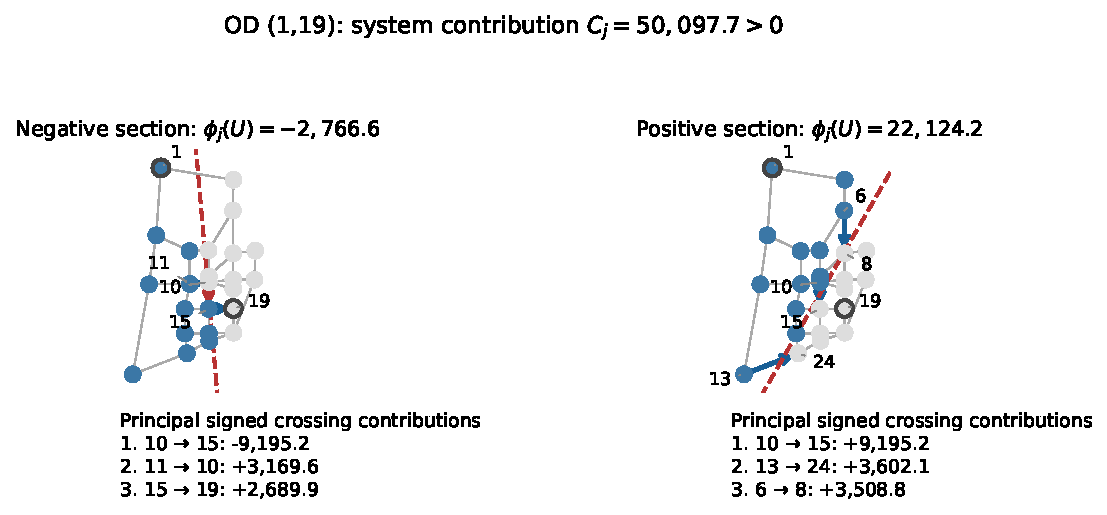
\includegraphics[width=0.99\linewidth]{../figures/fig_screenlines_v103.pdf}
\caption{Two straight screenlines for OD $(1,19)$, setting C. Blue nodes
belong to $U$; grey nodes are outside; dashed lines separate the two
sides. Node $1$ is inside and node $19$ outside in both panels. The two
accounts have opposite signs while the network-wide contribution is
positive. The lines are the minimum and maximum of the prespecified
geometric family; the complete irregular connected minimum and its
crossing-link decomposition appear in Figure~\ref{fig:negmech}.}
\label{fig:screenlines}\end{figure}


The enumerated extrema establish existence within the admissible
family; the prescribed boundaries separate sign from magnitude. All
tested origin-centred hop-distance and free-flow-time neighbourhood
accounts remain positive, yet within those families the largest account
is $8.9$, $9.0$, and $3.4$ times the smallest for $(1,19)$, $(1,15)$,
and $(7,12)$ (Appendix~\ref{supp:newodaccuracy}): sign stability does not mean that
simple, network-distance-defined boundaries give comparable magnitudes.
Straight screenlines sharpen the picture. Projecting the public node
coordinates onto $36$ pre-fixed directions ($5^\circ$ apart, both sides
of each line kept, positions midway between adjacent node projections,
connectedness and deduplication as in the connected family; no
attribution value enters the construction;
Appendix~\ref{supp:newodaccuracy}) yields $23$--$152$ distinct
straight-line boundaries per query. On these, $(1,19)$ and $(7,12)$
again attain negative accounts (minima $-2{,}767$ and $-2{,}967$ TSTT
units, on $2$ of $152$ and $10$ of $148$ boundaries), shallower than
the enumerated minima, while the remaining four queries in the screenline family stay
positive with magnitudes spanning up to a factor of $72$ for $(1,15)$
($511$--$36{,}621$). Practical straight-line sections therefore do not
inherit the sign safety of the neighbourhood families, nor do their
positive accounts agree in magnitude. Appendix~\ref{supp:newodaccuracy} reports the path-set, dispersion,
single-OD, and narrow-band checks. The separable TSTT structure gives a
particularly direct interpretation when only one demand changes:
\begin{equation}
\widetilde C_{e,j}=g_e(F_e^1)-g_e(F_e^0),\qquad g_e(F_e)=F_et_e(F_e).
\label{eq:edgeidentity}
\end{equation}
Indeed $dF_e/d\lambda=\Delta q_j\partial_jf_e$ along that path, so the
fundamental theorem of calculus applies link by link, including background
rerouting. Consequently $\phi_j(U)=H_U(f(q^1))-H_U(f(q^0))$: a negative
single-OD boundary account is an actual decrease in that signed boundary
cost sum. This identity also checks the numerical edge attribution directly.


\subsection{Input-stratified OD coverage}\label{sec:coverage_main}
An input-only stratified selection retains 18 of 528 positive Sioux Falls OD pairs, with two queries in each demand-by-free-flow-time tertile cell. Each OD varies alone over $\pm10\%$ and $\pm20\%$ intervals; other demands remain fixed with endogenous rerouting. The single-OD endpoint identity gives all edge accounts from four endpoint equilibria per query. Appendix~\ref{sec:coverage} reports the selection rule and all 18 queries.
\begin{table}[t]\centering\small
\caption{Input-stratified coverage across all 18 queries. Spreads use the Sioux Falls cost units. Ratios compare the pre-specified geometric family with all separating regions.}\label{tab:coverage_summary}
\begin{tabular}{lrrr}\toprule
Interval & Median geometric spread & Median unrestricted spread & Median ratio\\\midrule
$\pm10\%$ & 3292.5 & 7359.7 & 0.574\\
$\pm20\%$ & 6585.0 & 14719.5 & 0.574\\
\bottomrule\end{tabular}\end{table}
The geometric spread remains below the unrestricted spread for every selected query at both widths. The regional family therefore changes the magnitude of observed spatial variation. This fixed stratified sample is descriptive rather than a probability sample of demand conditions; same-state study/background decomposition is evaluated separately.

\subsection{External spatial calculation on Anaheim}\label{sec:anaheim}
The public Anaheim network has 416 nodes, 914 directed links and 1,406 positive OD demands \citep{tnfrc2024transportation}. We select the six largest demands, vary them jointly from 0.8 to 1.2 times their published values, and hold all other demands fixed while their route choices remain endogenous. Each OD uses ten free-flow shortest paths; candidate routes exclude other zone centroids as intermediate nodes (the first through node is 39). This reference calculation evaluates spatial computation and background mechanisms; no Anaheim surrogate is trained.
\begin{table}[t]\centering\small
\caption{Anaheim reference attribution (absolute accounts in vehicle-minutes per hour; divide by 60 for vehicle-hours per hour): unrestricted accounts and connected regions formed by removing edges on the OD path in two deterministic breadth-first spanning trees rooted at the origin and destination. These topology-only region rules use no attribution values. Ranges use 41-point integrated columns, with no connected-region enumeration.}\label{tab:anaheim}
\begin{tabular}{lrrrr}\toprule
OD & System & Unrestricted range & Selected connected range & Regions\\\midrule
(4,2) & 34664.1 & [-12712.6,20514.0] & [238.9,4932.1] & 36\\
(1,2) & 16773.6 & [-6032.2,9762.0] & [281.2,2964.7] & 26\\
(2,4) & 12143.7 & [-4374.6,6733.0] & [99.9,1915.3] & 36\\
(3,2) & 14706.7 & [-5613.8,9052.9] & [172.9,5777.4] & 28\\
(25,4) & 6919.3 & [-1805.3,3091.8] & [96.9,1212.2] & 22\\
(25,2) & 11445.9 & [-4157.3,6904.5] & [126.8,2676.4] & 16\\
\bottomrule\end{tabular}\end{table}
The reference chain with 21 quadrature states took 1278.7 seconds on the local CPU, including route construction and implicit sensitivities; the six unrestricted extrema took 0.0138 seconds after the columns were available. This separates the saved boundary-enumeration cost from reference attribution cost. Maximum path fixed-point residual was 1.1e-11, flow-balance residual 9.1e-12, and relative quadrature completeness discrepancy 3.2e-05.
At the common middle state, the six background-response norms range from 0.115 to 0.487, while their maximum node divergence is below $3.1\times10^{-15}$. Weighting those same responses by the common total-flow marginal costs gives divergence norms 0.116--0.796. Background rerouting therefore remains a nonzero spatial attribution mechanism on this larger network. 

For full-path mechanism analysis, order each query's pre-existing BFS regions lexicographically by its sorted node list and select the first, middle and last regions, denoted $U_0,U_1,U_2$. This rule uses topology and the OD only, without inspecting attribution. Each fixed comparison is decomposed using the same equilibrium states and total-flow marginal costs into free-flow/study, free-flow/background, congestion/study and congestion/background terms. Table~\ref{tab:anaheimmechanism} reports $\varphi_j(U_2)-\varphi_j(U_0)$; the additional $U_1-U_0$ comparisons and exact region memberships are archived with the experiment. These are differences for identical fixed regions, not sums of componentwise ranges.
\begin{table}[t]\centering\small
\caption{Anaheim full-path differences between two preselected connected regions (vehicle-minutes per hour). FF denotes free-flow costs, C congestion marginal costs, S the six study demands and B all other demands.}\label{tab:anaheimmechanism}
\begin{tabular}{lrrrrr}\toprule OD & FF/S & FF/B & C/S & C/B & Total\\\midrule
(4,2) & -0.00 & -0.10 & -1338.21 & 0.04 & -1338.28\\
(1,2) & 21.81 & 17.46 & 3.96 & -15.69 & 27.54\\
(2,4) & 0.00 & 0.00 & 654.99 & 0.00 & 654.99\\
(3,2) & 0.00 & -0.00 & -1622.92 & -0.00 & -1622.92\\
(25,4) & -396.00 & 4.26 & -673.82 & 1.47 & -1064.09\\
(25,2) & -412.24 & 0.49 & -2134.60 & 0.13 & -2546.22\\
\bottomrule\end{tabular}\end{table}
These mechanism columns use 41 equally spaced trapezoidal states. The maximum unrounded decomposition discrepancy is 9.1e-13 per edge. Refining from 21 to 41 states changes the node representation by relative Euclidean errors between 5.8e-06 and 5.2e-05 across queries; the largest selected-account change is 0.206 vehicle-minutes per hour (0.00452\% relative). This evaluates spatial accounts directly rather than relying on cancellation in scalar completeness. For $(1,2)$, the background free-flow term is positive whereas its congestion term is negative, and these contributions largely cancel. For most other selected comparisons the background terms are small relative to the study-response congestion term. The mechanism decomposition identifies both cancellation and relative magnitude under common total-flow cost weights.


\FloatBarrier
\section{Application to learned assignment}\label{sec:pairresults}
The spatial framework compares explanations produced by learned assignment
models with the reference equilibrium. We retain a final comparison of four
training objectives from the same five initial models, each continued for
1,200 updates under a shared validation rule. The 24 independent test paths
contain six each with one, two, three and six active OD queries. Statistics
average active queries and seeds within each path before summarizing paths;
training seeds do not increase the independent path count. Complete losses,
selection rules, costs and supplementary results appear in
Appendix~\ref{app:pairs-v102}; earlier comparisons are consolidated in
Appendix~\ref{app:legacy-learning}.
\begin{table}[t]\centering\small
\caption{Endpoint supervision on 24 independent paths (six each with one, two, three and six active OD queries), five seeds. Flow is the five-seed mean relative error on the original held-out demand states. Other entries first average active queries and seeds within each path, then report medians over paths; the last column gives the 90th percentile. All methods share 1,200 continuation updates and a common validation selection rule.}
\label{tab:pairs-v102}
\begin{tabular}{lrrrrrr}\toprule
Method & Flow (\%) & Column (\%) & System (\%) & Cut abs. & Cut (\%) & Cut P90 (\%)\\\midrule
Flow & 0.0386 & 21.61 & 2.33 & 270.16 & 14.53 & 34.27\\
Flow + endpoint edge & 0.0518 & 17.14 & 3.07 & 255.83 & 15.50 & 28.93\\
Flow + endpoint edge + cut & 0.0513 & 18.02 & 3.26 & 289.68 & 17.18 & 26.63\\
Flow + response & 0.0388 & 14.22 & 3.31 & 178.72 & 12.08 & 28.17\\
\bottomrule\end{tabular}\end{table}

Ordinary response supervision reduces median attribution-column error from
21.61\% to 14.22\% and boundary error from 14.53\% to 12.08\% relative to
flow supervision, reductions of 34.2\% and 16.9\%. These improvements belong
to established derivative supervision, not to a new training method proposed
here. Adding the endpoint boundary term gives 18.02\% column error and
17.18\% boundary error; its lower boundary 90th percentile does not establish
an overall advantage. Endpoint labels took 64.0 seconds versus 53.1 seconds
for center-state solves and response labels. The comparison demonstrates
that the spatial criteria distinguish explanation quality beyond flow fit,
while providing no overall accuracy or label-cost advantage for the added
boundary objective.

\section{Conclusions}\label{sec:conclusions}
Spatial OD accounts can be characterized, calculated and interpreted within
one framework. Their interchangeability depends jointly on network topology,
the query and the admissible region family. For two-sided connected regions,
only queried block paths constrain marginal outcome weights, allowing
heterogeneity elsewhere. For realized attributions, a node representation
supports selected-region comparison, unrestricted extrema, best common-value
approximation and exact model disagreement. Reusable projection scans extend
this computation to a specified finite family of straight screenlines.

Sioux Falls and Anaheim connect these calculations to traffic adjustment.
At common equilibrium states, crossing study and background responses with
free-flow and congestion weights identifies additive mechanisms behind
boundary differences. Positive network-wide contributions and negative
boundary accounts describe different, well-defined outcome changes. Learned
assignment provides a further use: spatial criteria reveal explanation
errors beyond flow-fit metrics, without requiring a new training algorithm
to outperform existing response supervision. The results apply to the fixed
road representations, prescribed region families and assignment models
stated here, and provide a basis for comparing spatial explanations of
traffic demand changes.

\section*{Code and data availability}
Experiment scripts, the numerical arrays behind the tables and figures,
and trained surrogate checkpoints are available from the corresponding
author on request. The requested package includes a README mapping
results to scripts and arrays.
The Sioux Falls and Anaheim networks and demands are available from the public
\href{https://github.com/bstabler/TransportationNetworks/tree/master/SiouxFalls}{Sioux Falls TNTP repository}
and \href{https://github.com/bstabler/TransportationNetworks/tree/master/Anaheim}{Anaheim TNTP repository}
\citep{tnfrc2024transportation}; training targets are synthetic fixed-path
logit-SUE assignments.
\section*{Declaration of competing interest}
The authors declare that they have no known competing financial interests
or personal relationships that could have appeared to influence the work
reported in this paper.
\FloatBarrier
\bibliographystyle{cas-model2-names}
\setlength{\bibsep}{0.8pt plus 0.2pt}
\bibliography{references_v103}
\appendix
\counterwithin{theorem}{section}
\counterwithin{rmk}{section}
\counterwithin{table}{section}
\counterwithin{figure}{section}
\counterwithin{equation}{section}
%% Mathematical appendix for the focused v82 revision.
\section{Mathematical foundations and proofs}\label{app:proofs}

\subsection{Conventions and conservation transfer}\label{app:notation}
The incidence matrix $B\in\R^{n\times m}$ has entries $-1$ at an arc's
origin and $+1$ at its destination; $\mu_j=e_{t_j}-e_{s_j}$ and
$M=[\mu_1,\ldots,\mu_K]$. Write $Z=\ker B$ and let $B^\dagger$ be the
Moore--Penrose pseudoinverse. All norms below are Euclidean or their
induced operator norms unless indicated otherwise. Graphs are loopless
multigraphs: parallel and reciprocal arcs remain distinct edges, including
in two-edge cycles. Cycle atoms and the block-cut tree are taken on the
underlying undirected multigraph. Formally, $\iota(v)$ is the cut-vertex
node when $v$ is an articulation vertex and otherwise its unique block
node; $\mathcal P(s,t)$ lists the atoms on the unique tree path from
$\iota(s)$ to $\iota(t)$. A signed simple $s$--$t$ path vector $p$ satisfies
$Bp=\mu$ and the full solution set is $p+Z$. Such a path uses only atoms
of $\mathcal P(s,t)$ and meets every atom on it.

\paragraph{Signed responses.}\label{app:signed}
The circulation and response vectors are signed first-order sensitivities,
not nonnegative commodity flows. At a strictly positive flow, sufficiently
small signed circulation perturbations also preserve nonnegativity. A
restricted response family is treated explicitly below.

\begin{corollary}[IG exchange]\label{cor:ig}
For an exactly conservative $C^1$ field on an open neighborhood of the
attribution path, $BG_{:,j}=\mu_j\Delta q_j$.
\end{corollary}
\begin{pf}
Differentiate $Bf(q)=Mq$ to obtain $BJ_f(q)=M$, then integrate the
$j$th column along $\gamma(\lambda)=q^0+\lambda\Delta q$.
\end{pf}

\subsection{Cycle structure and the classification proofs}\label{app:classificationproof}
\begin{lemma}[structure of circuit classes]\label{lem:mprime}
The non-bridge atoms are the non-singleton circuit classes; each bridge
is a singleton class. Moreover $Z=\bigoplus_A Z_A$, where
$Z_A=\{z\in Z:\operatorname{supp}z\subseteq A\}$, and the summands
have disjoint edge supports.
\end{lemma}
\begin{pf}
No simple cycle crosses an articulation vertex into another block: it
would revisit that vertex. Within a non-bridge block, any two edges lie
on a common cycle. One way to see this is to subdivide the two edges;
the resulting block is still biconnected, so its two new vertices lie
on a common cycle, which descends to the required cycle. This is the
usual circuit-class characterization of the graphic matroid
\citep{oxley2011matroid}. Every signed circulation is a linear combination
of signed simple-cycle vectors: subtract the fundamental cycles of a
spanning forest to leave a circulation on a forest, necessarily zero
by successive leaf elimination. Grouping these cycles by their blocks
gives the direct sum, and distinct blocks have disjoint edge sets.
\end{pf}

\begin{lemma}[circulation-preserving diagonal maps]\label{lem:m}
For $D=\operatorname{diag}(w)$, $DZ\subseteq Z$ if and only if $w$ is
constant on every non-bridge atom; bridge weights are free.
\end{lemma}
\begin{pf}
For any signed simple-cycle vector $z_C$, a circulation supported on
that cycle has equal signed amplitudes on successive edges, by node
balance. Thus $BDz_C=0$ forces $w$ constant on $C$, and
Lemma~\ref{lem:mprime} propagates equality throughout each atom.
Conversely, atomwise constancy makes $D$ a scalar on every $Z_A$, so
it preserves their direct sum. Bridges carry no circulation.
\end{pf}

\begin{pf}[Theorem~\ref{thm:t3cpmain}]
Add a virtual reverse OD edge $(t,s)$ and set
\[
\bar B=[B,-\mu],\qquad \bar D=\operatorname{diag}(w,\alpha).
\]
For a fixed $\alpha$, property~\eqref{eq:t3prop} is equivalent to
$\bar D\ker\bar B\subseteq\ker\bar B$.
Indeed, a kernel vector $(x,a)$ obeys $Bx=a\mu$. If $a\ne0$,
apply \eqref{eq:t3prop} to $x/a$ to obtain $BDx=a\alpha\mu$.
If $a=0$, subtract the identities for $p+x$ and $p$, with any fixed
$Bp=\mu$, to obtain $BDx=0$. These are exactly the two cases of
$\bar B\bar D(x,a)=0$. Conversely, applying kernel invariance to
$(x,1)$ gives \eqref{eq:t3prop} for every $Bx=\mu$, at that same $\alpha$.

By Lemma~\ref{lem:m}, this invariance holds precisely when the augmented
weights are constant on its cycle atoms. The virtual edge and a simple
$s$--$t$ path form a cycle meeting every original atom on
$\mathcal P(s,t)$, so these atoms merge with the virtual edge into one
circuit class. No other atoms join it: every new simple cycle contains
the virtual edge and a simple $s$--$t$ path, which uses only those
atoms. Other original atoms retain their classes. Thus the augmented
criterion is exactly within-atom constancy everywhere and common value
$\alpha$ on $\bigcup\mathcal P(s,t)$. This proves both directions and
identifies $\alpha=w^*$ without changing the universal response family.
\end{pf}

\begin{pf}[Theorem~\ref{thm:t3cm} and Corollary~\ref{cor:path}]
Apply the single-OD theorem to each query at the same $w$. Necessity
requires equality within every atom and among all atoms co-traversed
by a queried block path. Their transitive closure is exactly the
compatibility-class partition. Conversely, class constancy supplies
both single-OD conditions for every query. Along the attribution
path, exact conservation gives $BJ_f(\gamma(\lambda))\mathbf e_j=\mu_j$;
the static theorem therefore yields
\[
B\widetilde C_{:,j}=\Delta q_j\int_0^1
BD_\lambda J_f(\gamma(\lambda))\mathbf e_j\,d\lambda
=\Delta q_j\left(\int_0^1w^*_{k(j)}(\lambda)\,d\lambda\right)\mu_j.
\]
\end{pf}

\begin{corollary}[all-OD class collapse]\label{cor:allod}
Requiring the criterion at one common $w$ for every ordered pair of
distinct vertices makes all atoms in a connected component share one
constant.
\end{corollary}
\begin{pf}
For two atoms incident to the same cut vertex, choose endpoints on
their opposite sides. Their OD block path contains both atoms, forcing
their constants to agree. Connectivity of the block-cut tree propagates
the equality throughout the component.
\end{pf}

\begin{rmk}[a common flow realization]\label{rmk:quantifier}
The merging proof requires one common weight vector. Computing the
queries at different realized flows does not in general supply this
premise.
\end{rmk}

\subsection{Direction, integration, and network representation}\label{supp:criteria}
\begin{proposition}[universal directional criterion]\label{prop:directional}
Let $\hat x_j=B^\dagger\mu_j$, let $N$ span $Z$ with orthonormal
columns, and let $P_{\mu_j}$ project orthogonally onto
$\operatorname{span}\{\mu_j\}$. At fixed $w$, universal directional
balance is equivalent to
\[
(I-P_{\mu_j})BD\hat x_j=0,\qquad (I-P_{\mu_j})BDN=0.
\]
The scale may depend on the response. Requiring one common boundary value
additionally requires $BDN=0$. If directional balance holds along the
whole path for a conservative model, its integrated column balances.
\end{proposition}
\begin{pf}
Every response is $\hat x_j+z$, $z\in Z$. Apply $I-P_{\mu_j}$ to
$BD(\hat x_j+z)$ and vary $z$. The scale is
$\mu_j^\top BD(\hat x_j+z)/\norm{\mu_j}^2$ and is independent of
$z$ precisely when $BDZ=0$. Integrating the realized directional
identity gives the endpoint conclusion. Equivalently, invariance on
all incidence fibers, $Bx=By\Rightarrow BDx=BDy$, is exactly
$DZ\subseteq Z$, since $x-y$ ranges over $Z$.
\end{pf}

\begin{example}[strict separation of the criteria]\label{ex:triangle}
On the diamond $(s,a),(a,t),(s,b),(b,t)$ with weights $(1,1,1,2)$,
the upper-path response $(1,1,0,0)$ has divergence $\mu$ after
weighting, but the lower-path response has weighted divergence
$(-1,0,-1,2)$ in node order $(s,a,b,t)$, outside $\operatorname{span}\{\mu\}$.
On the triangle $(s,t),(t,u),(u,s)$ with weights $(1,0,0)$, every
response $x=(1+c,c,c)$ satisfies $BDx=(1+c)\mu$; direction balances,
but the common boundary value fails because the circulation $(1,1,1)$ maps
to $\mu\ne0$.
\end{example}

If directional balance holds for all
queries at common $w$, differences give
$BDZ\subseteq\bigcap_j\operatorname{span}\{\mu_j\}$. For non-collinear
queries this intersection is $\{0\}$, so directional balance implies
the common-value property. This uses the full response space $Z$.

\paragraph{Restricted families.}\label{app:membership}
For $S\subseteq Z$ with basis $N_S$, test responses in
$x_j^{\mathrm{ref}}+S$, where $Bx_j^{\mathrm{ref}}=\mu_j$.
The same proof gives the direction tests with $\hat x_j,N$ replaced
by $x_j^{\mathrm{ref}},N_S$; common boundary value replaces the second test by
$BDN_S=0$. Using $\hat x_j$ requires
$\hat x_j-x_j^{\mathrm{ref}}\in S$. For a fixed-path model $f=\Delta h$,
$A_{\mathrm{OD}}h(q)=q$ and $B\Delta=MA_{\mathrm{OD}}$. Choose a path
vector $a_j$ with $A_{\mathrm{OD}}a_j=\mathbf e_j$ and set
$x_j^{\mathrm{ref}}=\Delta a_j$. Differentiation yields
\[
J_f\mathbf e_j-x_j^{\mathrm{ref}}
=\Delta(\partial_jh-a_j)\in\Delta\ker A_{\mathrm{OD}}=:T_{\mathrm{swap}}.
\]
This space includes same-OD path exchanges of every OD: background
ODs may reroute even when their demands remain fixed.

\begin{example}[endpoint cancellation]\label{ex:cancellation}
For two series bridges, $f(q)=(q,q)$ and
$T(F)=F_1+F_2+[\sin(2\pi F_1)-\sin(2\pi F_2)]/(2\pi)$ give
\[
\widetilde C_1-\widetilde C_2
=\frac{\sin(2\pi q^1)-\sin(2\pi q^0)}{\pi}.
\]
For $q^0=0$, the nonzero balanced endpoints in $[0,1]$ are
$q^1=1/2,1$, although the two marginal weights differ almost
everywhere. At $q^1=0.3$ balance fails. Endpoint cancellation therefore
does not establish the pointwise classification conditions.
\end{example}

\begin{example}[network subdivision]\label{ex:subdivision}
A single edge with $f(q)=q$, $T(F)=\tau F$, $\tau>0$, has cut account
$\tau\Delta q$. Subdivide it into $(s,v),(v,t)$ and set
$f'(q)=(q,q)$,
$T'(F_1,F_2)=\tau[\alpha F_1+(1-\alpha)F_2]$, $0<\alpha<1$.
The composite demand-to-outcome map is unchanged, but
$\widetilde C'=\tau\Delta q(\alpha,1-\alpha)$ and
$(B\widetilde C')_v=\tau(2\alpha-1)\Delta q$.
The two cuts account $\tau\alpha\Delta q$ and
$\tau(1-\alpha)\Delta q$. They agree only for $\alpha=1/2$, when each
is half the undivided account; their sum remains the scalar
contribution $\tau\Delta q$. The invariance studied here thus concerns
conservative responses on a fixed network with a fixed edgewise
outcome definition, rather than invariance under subdivision.
\end{example}

\subsection{Approximate conservation and attribution balance}\label{app:approx}
\label{app:failurestatement}
\begin{theorem}[Failure of attribution balance under approximate conservation]\label{thm:t1mmain}
Fix $\varepsilon>0$ and $\delta\ne0$. With input dimension $K=2$ and
$v\in\operatorname{im}(B)$, $\norm{v}=1$, there is an analytic
demand-to-flow map
$f_\varepsilon:\R^2\to\R^m$ (constructed in
Appendix~\ref{app:proofs}) such that
\[
\sup_{q\in\R^2}\norm{r_\varepsilon(q)}\le\varepsilon,
\qquad\text{with } r_\varepsilon\equiv0
\text{ on the diagonal set } \{q:q_1=q_2\},
\]
yet along the diagonal path $q(\lambda)=\lambda(\delta,\delta)$ its
per-column attribution residuals are
\[
R_1=v\,\delta,\qquad R_2=-v\,\delta:
\ \text{\emph{fixed scale $|\delta|$, independent of $\varepsilon$}} .
\]
\end{theorem}

\paragraph{Proof of Theorem~\ref{thm:t1mmain}.}\label{app:tanhfamily}
For $K=2$ and $\norm v=1$, $v\in\operatorname{im}B$, set
\[
r_\varepsilon(q)=\varepsilon v\tanh((q_1-q_2)/\varepsilon),
\qquad f_\varepsilon(q)=B^\dagger(Mq+r_\varepsilon(q)).
\]
Since $BB^\dagger$ projects onto $\operatorname{im}B$, the residual
of this analytic field is exactly $r_\varepsilon$, bounded globally
by $\varepsilon$ and zero on $q_1=q_2$. Writing
$x=(q_1-q_2)/\varepsilon$ gives
$J_{r_\varepsilon}=v\operatorname{sech}^2(x)(1,-1)$.
On $q(\lambda)=\lambda(\delta,\delta)$, $x=0$, so the residual identity
\eqref{eq:residualidentity} yields $R_1=\delta v$, $R_2=-\delta v$.
The second derivatives are bounded above by $C/\varepsilon$ and
attain magnitude $c/\varepsilon$ at a fixed nonzero $x$; thus
$\mathrm{Lip}(J_{r_\varepsilon})\asymp\varepsilon^{-1}$.
\hfill$\square$

\begin{proposition}[strictly positive strengthening]\label{prop:positive}
Let $K\ge2$, $Q=[\ell,u]^K\subset(0,\infty)^K$, and let $f_0$ be
exactly conservative and $C^1$ near $Q$, with
$\varrho=\min_{q\in Q,e}(f_0(q))_e>0$. For unit
$v\in\operatorname{im}B$, define
$f_\varepsilon=f_0+B^\dagger r_\varepsilon$ with the same
$r_\varepsilon$ as above. Its residual is bounded by $\varepsilon$
and vanishes on $q_1=q_2$. If
$\varepsilon<\varrho/\norm{B^\dagger}_2$, all flows stay strictly
positive. Along any path
$q^0+\lambda\delta(\mathbf e_1+\mathbf e_2)\subset Q$ with
$q^0_1=q^0_2$, its column residuals are $R_1=\delta v$,
$R_2=-\delta v$, independent of $\varepsilon$.
\end{proposition}
\begin{pf}
The projection identity gives the residual exactly, while
$\norm{f_\varepsilon-f_0}_\infty\le
\norm{B^\dagger}_2\varepsilon<\varrho$ preserves positivity.
On the diagonal path the first two partial derivatives of the
residual are $v,-v$. Integrate them; the exactly conservative
$f_0$ contributes zero residual. The normalized residual is therefore
$\norm{R_j}/(|\Delta q_j|\norm{\mu_j})=1/\norm{\mu_j}$.
\end{pf}

\begin{theorem}[local neighborhood bound]\label{thm:t1pmain}
Let $r\in C^{1,1}(\mathcal N;\R^n)$ on an open neighborhood of the
attribution path, with $\operatorname{Lip}(J_r)\le H$.
Suppose, for some $\rho>0$ and every $j,\lambda$,
$\gamma(\lambda)+[-\rho,\rho]\mathbf e_j\subset\mathcal N$ and
$\|r(\gamma(\lambda)\pm\rho\mathbf e_j)\|\le\varepsilon$.
Then
\[
\|R_j\|\le|\Delta q_j|(\varepsilon/\rho+H\rho/2).
\]
\end{theorem}
\paragraph{Proof of Theorem~\ref{thm:t1pmain}.}\label{app:stencil}
For $q=\gamma(\lambda)$, the hypotheses place
$q+[-\rho,\rho]\mathbf e_j$ inside $\mathcal N$. Taylor's formula with a
Lipschitz Jacobian gives
$r(q\pm\rho\mathbf e_j)=r(q)\pm\rho\partial_jr(q)+\xi_\pm$,
$\norm{\xi_\pm}\le H\rho^2/2$. Subtracting the two formulas and
using the endpoint residual bounds yields
$\norm{\partial_jr(q)}\le\varepsilon/\rho+H\rho/2$.
Integrating \eqref{eq:residualidentity} proves the claim.
\hfill$\square$

\begin{rmk}[Sharpness of the square-root rate]\label{rmk:sqrttight}
The rate in Theorem~\ref{thm:t1pmain} cannot be uniformly improved within
its own hypothesis class. With $K=2$, unit $v\in\operatorname{im}(B)$, and
\[
r_\varepsilon(q)=\varepsilon v\sin\!\big((q_1-q_2)/\sqrt\varepsilon\big),
\qquad
f_\varepsilon(q)=B^\dagger\big(Mq+r_\varepsilon(q)\big),
\]
the projection identity of the proof of Theorem~\ref{thm:t1mmain} gives
output residual exactly $r_\varepsilon$, so
$\sup_q\norm{r_\varepsilon(q)}\le\varepsilon$. Moreover
\[
J_{r_\varepsilon}(q)
=\sqrt\varepsilon\,v\cos\!\big((q_1-q_2)/\sqrt\varepsilon\big)(1,-1),
\qquad
\mathrm{Lip}(J_{r_\varepsilon})\le2
\]
for every $\varepsilon$: the hypotheses hold with $\mathcal N=\R^2$,
$H=2$, and any $\rho>0$, uniformly in $\varepsilon$. Along the diagonal
path $q(\lambda)=\lambda(\delta,\delta)$ the derivative evaluates to
$\sqrt\varepsilon\,v(1,-1)$, so the residual
identity~\eqref{eq:residualidentity} gives
\[
R_1=\delta\sqrt\varepsilon\,v,\qquad R_2=-\delta\sqrt\varepsilon\,v,
\]
of exact order $\sqrt\varepsilon$. Within the class of residuals with
residual bound $\varepsilon$ and bounded Jacobian Lipschitz constant, no
uniform $o(\sqrt\varepsilon)$ refinement of Theorem~\ref{thm:t1pmain} is
therefore possible; the exponent, not merely the constant, is sharp.
\end{rmk}

\begin{lemma}[minimum-norm support]\label{lem:s}
For a signed $s$--$t$ path $p$, $\hat x=B^\dagger\mu=(I-P_Z)p$
is supported on $\bigcup\mathcal P(s,t)$.
\end{lemma}
\begin{pf}
The minimum-norm point of $p+Z$ is its orthogonal projection onto
$Z^\perp$. Lemma~\ref{lem:mprime} gives
$P_Z=\sum_A P_{Z_A}$ with disjoint supports; both $p$ and every
$P_{Z_A}p$ vanish on off-path atoms.
\end{pf}

\begin{proposition}[combined dispersion--residual bound]\label{prop:combined}
Let $f\in C^1$ near the attribution path, $r=Bf-Mq-b$ with the constant
background balance $b$ of Section~\ref{sec:noninheritance} ($b=0$
without background), and let
$w(\lambda)=\nabla T(f(\gamma(\lambda)))$ be continuous.
Let $\bar w(\lambda)$ be the compatibility-class mean vector and
$\eta(\lambda)=\norm{w(\lambda)-\bar w(\lambda)}_\infty$.
Writing $J_j(\lambda)=J_f(\gamma(\lambda))\mathbf e_j$ and
$d_j=(I-P_{\mu_j})B\widetilde C_{:,j}$, we have
\[
\norm{d_j}_2\le |\Delta q_j|\norm{B}_2\int_0^1\left[
\eta(\lambda)\norm{J_j(\lambda)}_2+
\norm{\bar w(\lambda)}_\infty\norm{B^\dagger}_2
\norm{\partial_jr(\gamma(\lambda))}_2\right]d\lambda.
\]
\end{proposition}
\begin{pf}
Differentiation gives $BJ_j=\mu_j+\partial_jr$ --- $b$ is constant and
drops out of the derivative --- so
$J_j=\hat x_j+z_j+B^\dagger\partial_jr$, $z_j\in Z$.
Let $\bar D=\operatorname{diag}(\bar w)$. Class constancy gives
$B\bar Dz_j=0$ by Lemma~\ref{lem:m}. By Lemma~\ref{lem:s},
$\hat x_j$ is supported on the OD block path, whose atoms lie in one
compatibility class $k(j)$; hence
$B\bar D\hat x_j=\bar w_{k(j)}\mu_j$.
Therefore
\[
(I-P_{\mu_j})BDJ_j=(I-P_{\mu_j})B
\left[\operatorname{diag}(w-\bar w)J_j+
\bar DB^\dagger\partial_jr\right].
\]
The projector is non-expansive, the two diagonal operator norms are
$\eta$ and $\norm{\bar w}_\infty$, and integration gives the bound.
For exact conservation only the dispersion term remains; for
$\eta=0$ only the derivative residual remains. Theorem~\ref{thm:t1pmain}
can bound that derivative term under its local hypotheses.
\end{pf}

\subsection{Exact boundary error and its path bound}\label{app:boundaryerror}
\begin{pf}
Set $b=Be_j$ and $I=V\setminus\{s_j,t_j\}$. Since $\mathbf1^\top b=0$,
Eq.~\eqref{eq:cutextrema} applied to $e_j$ gives an interval of extrema
with midpoint
\[
-b_{s_j}-\frac12\sum_{v\in I}b_v
=\frac12(b_{t_j}-b_{s_j})
\]
and half-width $\frac12\sum_{v\in I}|b_v|$. The larger absolute
endpoint is the absolute midpoint plus this half-width, proving
Eq.~\eqref{eq:exactboundaryerror}. This argument concerns the attained
extrema; it does not require every value between them to be attained.
The map $\mathcal K_j$ is a seminorm because it is a sum of absolute
linear functionals. Moreover
$e_j=\Delta q_j\int_0^1 h_j(\gamma(\lambda))\,d\lambda$.
Its homogeneity and triangle inequality therefore yield
\[
\epsilon_j^{\mathcal U}\le\mathcal K_j(e_j)
\le |\Delta q_j|\int_0^1\mathcal K_j(h_j(\gamma(\lambda)))\,d\lambda,
\]
proving the path statement. Its kernel is $\ker B$: if the seminorm
vanishes, all interior divergences vanish and $b_{s_j}=b_{t_j}$;
the zero sum then makes both endpoints zero.
\end{pf}


\subsection{Connected-region classification}\label{app:connectedproof}
We retain the loopless multigraph conventions of
Appendix~\ref{app:notation}; reciprocal arcs are distinct undirected
edges when defining atoms and connectivity.

\begin{lemma}[localization of a separating bond]\label{lem:bondlocal}
If $G[U]$ and $G[V\setminus U]$ are connected, all edges of
$\delta(U)$ lie in one cycle atom (or its singleton bridge).
If $s\in U$ and $t\notin U$, that atom lies on $\mathcal P(s,t)$.
\end{lemma}
\begin{pf}
For two distinct crossing edges, connect their endpoints by a simple
path inside $U$ and by another inside its complement. The two paths
have disjoint vertex sets; together with the crossing edges they form
a simple cycle, including the possible two-edge cycle. Hence all
crossing edges share a circuit class. A singleton crossing edge is a
bridge. A simple $s$--$t$ path crosses this boundary, so it meets its
atom; every atom met by such a path lies on $\mathcal P(s,t)$.
\end{pf}

\begin{lemma}[connected prefixes in an atom]\label{lem:prefixatom}
Let $A$ be a non-bridge atom and let $a\ne b$ be two of its vertices.
Its vertices admit an ordering $v_1=a,\ldots,v_k=b$ such that every
proper nonempty prefix and its suffix induce connected subgraphs.
The assertion includes two-vertex parallel-edge atoms.
\end{lemma}
\begin{pf}
For two vertices the assertion is immediate. Otherwise add an $a$--$b$
edge temporarily if needed. The connected-prefix property is the classical
$st$-numbering property \citep{even1976st}; we give a construction here.
A biconnected graph with this edge admits
an open-ear construction starting from a cycle containing that edge.
For completeness, this construction follows directly from vertex
connectivity. If vertices remain outside the current subgraph, any
component of those vertices has at least two distinct attachment
vertices in the current subgraph: a unique attachment would be an
articulation of the original graph. A path through the component
between two attachments supplies the next ear. Repeat until all
vertices have entered. Edges left over are irrelevant to the ordering.
The initial cycle exists because the added edge is not a bridge.

Order the other arc of the initial cycle from $a$ to $b$. For each
subsequent ear, let $u$ precede $v$ among its two attachment vertices;
insert its internal vertices, in their order from $u$ to $v$,
immediately after $u$. Every new internal vertex has an earlier and a
later neighbor. Existing vertices keep these neighbors. The first and
last vertices remain $a,b$. Every vertex except $a$ therefore has an
earlier neighbor and every vertex except $b$ a later neighbor. Repeated
steps along these neighbors connect every prefix to $a$ and every
suffix to $b$. Removing the temporary edge does not affect this
argument: it is never internal to a proper prefix or suffix.
\end{pf}

\begin{pf}[Theorem~\ref{thm:connectedclassification}]
For sufficiency, Lemma~\ref{lem:bondlocal} places every crossing edge
in one traversed atom. Its weight is $\alpha$, so
$-\mathbf1_U^\top BDx=-\alpha\mathbf1_U^\top Bx
=-\alpha\mathbf1_U^\top(e_t-e_s)=\alpha$.
No other edge enters this boundary sum.

For necessity, fix a traversed atom $A$. Delete its edges but keep its
vertices. The remaining graph has one connected component $T_v$ for
each $v\in V(A)$, containing that vertex and no other vertex of $A$.
Indeed an outside path between two vertices of $A$ would join their
blocks in a cycle, contrary to the block-cut tree. Connectivity of $G$
shows these components partition $V$. There are distinct vertices
$a,b$ with $s\in T_a$ and $t\in T_b$; these are the entry and exit of
the OD block path in $A$. For a bridge, take the cut consisting of
its $s$-side component. Since its unit conservative crossing response
is fixed, the assumed account immediately gives that bridge's weight
$\alpha$.

For a non-bridge atom, choose the ordering of
Lemma~\ref{lem:prefixatom}. Set
$U_i=\bigcup_{\ell\le i}T_{v_\ell}$ for $1\le i<k$.
The bags and the prefix/suffix connectivity show
$U_i\in\mathcal U^{\mathrm{conn}}_{st}$. Its crossing edges are exactly
those of the corresponding prefix in $A$.
Now choose any signed local response $y$ with
$B_Ay=e_b-e_a$, where $B_A$ is the incidence matrix on $A$.
Extend it by a signed unit path from $s$ to $a$ inside $T_a$ and from
$b$ to $t$ inside $T_b$, with zero on other edges. The result satisfies
$Bx=\mu$. Thus the assumption gives
\[
-\sum_{\ell\le i}(B_AD_Ay)_{v_\ell}=\alpha
\quad(1\le i<k).
\]
The first prefix gives $(B_AD_Ay)_a=-\alpha$, differences of consecutive
prefixes give zero at every interior vertex, and zero total incidence
sum gives $(B_AD_Ay)_b=\alpha$. Consequently
$B_AD_Ay=\alpha(e_b-e_a)$ for every local conservative $y$.
The single-OD classification (Theorem~\ref{thm:t3cpmain}), applied to the
one-atom graph $A$, forces every edge in $A$ to have weight $\alpha$.
This holds for every traversed atom. The sufficiency argument already
shows that no off-path weight is constrained.
\end{pf}

\begin{pf}[Corollary~\ref{cor:connectedmulti}]
Apply Theorem~\ref{thm:connectedclassification} at the common $w$ to
each query. Each queried path requires one weight on all its edges;
intersecting paths propagate equality transitively. Conversely these
transitive equalities satisfy every single-query condition. Atoms not
on any queried path enter none of these equalities.
\end{pf}

\subsection{Finite-change supervision and joint-path implication}\label{app:pairproof}
\begin{pf}[Proposition~\ref{prop:pairboundary}]
Write $r\in\{L,S\}$ and $c^r(q)=g(f^r(q))$ componentwise. Along a
single-coordinate segment $q(u)=q^-+u(q^+-q^-)$, the chain rule gives
\[
\frac{d}{du}c^r(q(u))=(q_j^+-q_j^-)
D^r(q(u))J_j^r(q(u)).
\]
Integration gives the attribution column exactly as
$\widetilde C^r_{:,j}=c^r(q^+)-c^r(q^-)=z_j^r$.
Corollary~\ref{cor:boundaryerror} applied to their difference proves
the stated maximum-error identity. No reference input derivative is
needed to obtain this label.

For the local-to-joint implication set
$A(q)=B[c^L(q)-c^S(q)]$. Equality of every separating boundary account
of a sufficiently small single-coordinate change implies
$\mathcal K_j(c^L(q+\epsilon e_j)-c^L(q)
-c^S(q+\epsilon e_j)+c^S(q))=0$.
The seminorm's kernel is $\ker B$: its expression forces all internal
entries of $Bh$ to vanish and its two endpoint entries to agree; their
zero total then forces both to vanish. Hence
$A(q+\epsilon e_j)=A(q)$. Differentiability and division by $\epsilon$
yield
\[
\partial_j A(q)=B[D^L(q)J_j^L(q)-D^S(q)J_j^S(q)]=0.
\]
On any valid joint attribution path, integration of this identity gives
zero divergence of the corresponding attribution-column error, and
therefore matching accounts on every separating boundary. This needs
the local matching premise throughout the domain containing the path;
a finite training sample supplies no such premise.
\end{pf}

\section{Experimental methods}\label{supp:fields}\label{supp:metrics}
\subsection{Network, path sets, and demand settings}\label{supp:networks}
The public Sioux Falls network has $24$ nodes and $76$ directed arcs
\citep{tnfrc2024transportation}. All arcs belong to one cycle atom, hence
one compatibility class. The eight queries are the positive-demand OD pairs with the largest
published demands, with ties broken by ascending origin then destination
node ID. All happen to involve node $10$.
The queries are
$(10,16)$, $(16,10)$, $(10,11)$, $(10,15)$, $(15,10)$, $(10,17)$, $(11,10)$, $(17,10)$,
with published demands
$q_{\mathrm{base}}=(4400,4400,4000,4000,4000,3900,3900,3900)$ veh/h.
The attribution path changes these demands from $0.2q_{\mathrm{base}}$ to
$1.6q_{\mathrm{base}}$. Node IDs in the traffic experiments are one-based.
Flows retain the benchmark's approximate-hourly convention; one time unit
is $0.01$ h. A reported TSTT number is $\sum_e F_et_e(F_e)$ with $F_e$
in veh/h and $t_e$ in these time units: multiplying by $0.01$ gives the
hourly vehicle-hour total, without extrapolating to a day. All absolute
attribution and boundary-account numbers use the same convention.

For each OD we retain every loopless directed path if enumeration finishes
within $200$ paths, otherwise the ten shortest by free-flow cost (Yen's
algorithm, lexicographic edge-sequence tie breaking); no OD in this
network has a fully enumerated set under the threshold. All eight query
ODs use ten paths. The link--path incidence $\Delta$ and the matrix $A$
summing paths within each OD stay fixed, so $B\Delta=MA$ with the
appropriate full or study OD incidence matrix. The full-background
ten-path set has $5{,}280$ paths (ten per OD; the expanded set
$10{,}560$, twenty per OD); Appendix~\ref{supp:coverage} compares these
candidate-path models.

The path-exchange response space $T_{\mathrm{swap}}=\Delta\ker A$
(Appendix~\ref{app:membership}) has dimension $32$ in A with ten
paths for each study OD, and dimension $53$ in C with either ten or
twenty paths for every OD, equal to the full circulation-space
dimension $m-n+1=53$ (ranks computed from within-OD differences of
link--path incidence columns). Full background therefore spans the
complete circulation space through allowable path exchanges, while
the eight-OD path model spans a proper subspace.

The three demand settings share the same query endpoints. In setting A,
all other demands are zero. In setting B, assign all positive
background demands jointly with the study demands fixed at
$q^0=0.2q_{\mathrm{base}}=(880,880,800,800,800,780,780,780)$ veh/h in
the listed query order, freeze the resulting background link flows, and
re-equilibrate only the eight query ODs. In setting C, the other $520$
positive OD demands stay at published values while all $528$ ODs
re-equilibrate jointly at every path point and perturbation. TSTT and
its gradient use total link flows in B and C; setting C is a
full-background assignment with eight attribution queries, not an
attribution evaluation of all $528$ ODs.

\subsection{Equilibrium and its sensitivities}\label{supp:sue}
Unless stated otherwise, the fixed-path logit stochastic user equilibrium
(SUE) uses $\theta=1$ and BPR costs
$t_e(F_e)=t_{0,e}[1+0.15(F_e/c_e)^4]$. With $\Pi_j$ the path set,
\begin{equation}
h_p=q_jp_p(F),\quad
p_p(F)=\frac{\exp[-\theta(\Delta^\top t(F))_p]}
{\sum_{r\in\Pi_j}\exp[-\theta(\Delta^\top t(F))_r]},\quad
F=\Delta h.\label{eq:sueloading}
\end{equation}
This is the solution of
\[
\min_{h\ge0,\ Ah=q}\left\{
\sum_e\int_0^{(\Delta h)_e}t_e(s)ds+
\theta^{-1}\sum_p h_p(\log h_p-1)\right\}.
\]
For positive demands the feasible set is nonempty and compact and the
objective strictly convex. A zero path flow can be improved by transferring
mass from a positive path of the same OD, since the entropy change is
$\theta^{-1}\epsilon\log\epsilon+O(\epsilon)<0$; hence the minimizer is
positive. Its Hessian and sensitivity equations are
\begin{equation}
H=\Delta^\top\operatorname{diag}(t'_e)\Delta+
\theta^{-1}\operatorname{diag}(1/h_p)\succ0,\qquad
\begin{bmatrix}H&A^\top\\A&0\end{bmatrix}
\begin{bmatrix}\partial_jh\\\partial_j\nu\end{bmatrix}
=\begin{bmatrix}0\\\mathbf e_j\end{bmatrix}.
\label{eq:kkt_sensitivity}
\end{equation}
$A$ has full row rank, so the system is nonsingular and the implicit
function theorem gives a $C^1$ demand-to-flow map.

For background re-routing we solve the equivalent total-link-flow fixed
point $F=L(F,q)=\Delta\{q_jp_{\Pi_j}(F)\}_j$ by Newton steps with residual
line search. For frozen background the corresponding equation is
$F=F_{\mathrm{bg}}^0+\Delta_{\mathrm{study}}
\{q_jp_{\Pi_j}(F)\}_{j\in\mathrm{study}}$, where $F_{\mathrm{bg}}^0$
is fixed at the joint $q^0$ equilibrium. Costs and gradients use this
total $F$ in both equations. Every solution is checked against its path-loading
equation, with maximum absolute path-flow gap below $10^{-7}$ veh/h.
The $76$-dimensional implicit system avoids forming a dense path Hessian.
For an OD group $R$, define
\[
S_R=\theta\sum_{k\in R}\Delta_k
\left[\operatorname{diag}(h_k)-h_kh_k^\top/q_k\right]\Delta_k^\top,
\quad W=\operatorname{diag}(t'_e(F_e)),\quad S=S_{\mathrm{all}}.
\]
Differentiating the logit probabilities gives
$\partial_F L_R=-S_RW$. Consequently the total sensitivity satisfies
\begin{equation}
(I+SW)J_j=\Delta_jp_j,\qquad
J_j^{\mathrm{study}}=\Delta_jp_j-S_{\mathrm{study}}WJ_j,\qquad
J_j^{\mathrm{bg}}=-S_{\mathrm{bg}}WJ_j.
\label{eq:bg_sensitivity}
\end{equation}
Here ``study'' includes all eight queried ODs and ``background'' the
other $520$: $J_j=J_j^{\mathrm{study}}+J_j^{\mathrm{bg}}$,
$BJ_j^{\mathrm{study}}=\mu_j$, $BJ_j^{\mathrm{bg}}=0$, the study
term including responses of the other seven study ODs. The
decomposition uses one joint equilibrium, rather than sensitivities
at different congestion states.
For setting B the background flows have no derivative, so the same
implicit system uses $S=S_{\mathrm{study}}$, with
$J_j^{\mathrm{study}}=J_j$ and $J_j^{\mathrm{bg}}=0$.

Central finite differences independently re-solve Eq.~\eqref{eq:sueloading}
at $q\pm a_j\mathbf e_j$, $a_j=0.005q_{\mathrm{base},j}$ and
$a_j/2$; both steps are checked at every $\theta=1$ ten-path
re-routing integration point, the path-set and $\theta$ variations
add half-step checks for all eight columns at the path midpoint, and
the link Newton solver is compared against the successive-averages
background equilibria at their common eleven quadrature points.

\subsection{Conservative learned surrogate}\label{supp:protocol}
The zero-background surrogate parameterizes
$h_j=q_j\operatorname{softmax}(z(q)|_{\Pi_j})$, $f=\Delta h$.
The three hidden layers each have $128$ tanh units; the final layer is
linear. The logit head uses training-standardized demands while the raw
$q_j$ multiplies the shares, preserving nonnegative flow and exact
conservation. Computations use double precision.
Training targets are fixed-path logit-SUE assignments ($\theta=1$,
path fixed-point tolerance $10^{-6}$). The $2500/857/857$
training/validation/test split uses seed $20260820$, with demands
$q_j=q_{\mathrm{base},j}s_j$ and independent $s_j$ drawn from
LogNormal$(0,0.5^2)$ clipped to $[0.2,2]$.
Adam uses learning rate $0.003$, full-batch link-flow MSE, at most
$12{,}000$ steps, and validation every $50$ steps. The
minimum-validation-error state of each seed $0,\ldots,4$ supplies
the reported results, with automatic differentiation supplying their
Jacobians; the test split is used only for final reporting.

\subsection{Integration grids, connected boundaries, and cancellation diagnostics}\label{supp:quadrature}
All numerical integrations use composite trapezoids. The principal
learned zero-background results use $201$ quadrature points; direct
zero-background SUE and both background settings use $41$ in the main
table. Frozen background compares $11$ with $41$ points; re-routing
compares $11$, $21$, and $41$ nested points; the two near-balanced
queries add $81$ and $161$ nested points; the learned-versus-SUE
sensitivity comparison uses identical $41$-point grids, kept separate
from the $201$-point learned results (Appendix~\ref{supp:accuracy}).

Connected boundaries require both $G[U]$ and $G[V\setminus U]$ to be
connected on the underlying undirected graph, with $s_j\in U$, $t_j\notin U$.
Exact enumeration yields $10{,}270$--$13{,}253$ admissible sets for each
of the eight main study ODs, and $4{,}621$--$16{,}943$ for the six
additional queries of Appendix~\ref{supp:newod}.
Extrema of $-\mathbf1_U^\top B\widetilde C_j$ are evaluated by exact
enumeration, cross-checked against independent subset enumeration on
restricted neighborhoods; attaining sets are verified for membership
with values recomputed by direct summation. These are connected
regions, not claimed to be administrative boundaries.

For cancellation diagnostics define
$A_j=|\Delta q_j|\int_0^1\sum_{v\notin\{s_j,t_j\}}|(BD_\lambda J_j)_v|d\lambda$
and $\kappa_j=1-S_j/A_j$ when $A_j>0$. The triangle inequality gives
$0\le S_j\le A_j$. Both quantities use the specified $201$-point learned
grid and are summarized over the five seeds; checks on additional
path-set or dispersion models sample the demand-path midpoint and
endpoints.

\subsection{Six pre-specified queries away from node 10}\label{supp:newod}
The selection rule uses only published demands and free-flow
shortest-path times. Candidates are the positive-demand ODs whose origin
and destination both differ from node $10$; ranking them by demand and
splitting into three equal-count terciles, the minimum- and
maximum-free-flow-shortest-path OD within each tercile is selected, with
ties broken by ascending (origin, destination). The six queries are
$(7,18)$, $(1,19)$, $(4,5)$, $(1,15)$, $(6,8)$, and $(7,12)$, with
published demands $(200,300,500,500,800,700)$ veh/h and free-flow
shortest-path times $(2,22,2,23,2,19)$ time units; the joint
protocol, sensitivities, and boundary enumeration are as in
Section~\ref{subsec:newod}, with conservation checks at setting-C
floating-point levels (maximum path fixed-point residual
$1.6\times10^{-10}$ veh/h, midpoint implicit-versus-finite-difference
column error $2.6\times10^{-8}$, completeness $4.3\times10^{-7}$).

For the single-OD checks, let $\bar q=q^{\mathrm{base}}$ be the full
published demand vector over all $528$ positive-demand ODs. For each
focal query $j\in\{(1,19),(1,15),(7,12),(6,8)\}$, define
\begin{equation}
q^{(a)}=\bar q+(a q_j^{\mathrm{base}}-\bar q_j)e_j,
\qquad
q^{(b)}=\bar q+(b q_j^{\mathrm{base}}-\bar q_j)e_j,
\qquad
(a,b)\in\{(0.2,1.6),(0.9,1.1),(0.8,1.2)\},
\label{eq:singleodstates}
\end{equation}
where $e_j$ is the coordinate unit vector. All other $527$ demands,
including the other five selected queries, remain at their published
values $\bar q_{-j}$ along the segment. Direct equilibria and the learned
small-band checks use these same reference states. The setting-C solver,
path sets, and boundary definitions are unchanged; checks and interval
results are in Appendix~\ref{supp:newodaccuracy}. For each interval,
Eq.~\eqref{eq:edgeidentity} gives the attribution column from the two
endpoint equilibria alone.


\subsection{Anaheim network, equilibrium and predefined regions}\label{app:anaheimsettings}
Both network and demand files are the public Transportation Networks for Research Core Team Anaheim TNTP data \citep{tnfrc2024transportation}. The network header supplies free-flow times in minutes and capacities in vehicles per hour; all roads use the published BPR coefficient 0.15 and power 4. We use $t_e(F_e)=t_e^0[1+0.15(F_e/c_e)^4]$ and TSTT marginal weight $t_e^0[1+0.75(F_e/c_e)^4]$. The six study OD demands, ranked by descending base demand and then lexicographic OD, are $(4,2)$: 2106.7, $(1,2)$: 1365.9, $(2,4)$: 1271.4, $(3,2)$: 1237.9, $(25,4)$: 1232.4, $(25,2)$: 1232.3 vehicles per hour. They move jointly from 0.8 to 1.2 times base demand; all remaining positive demands stay at their published base values and retain endogenous route choice. Every OD uses ten loopless free-flow shortest routes from Yen's algorithm. Ties within $10^{-12}$ minutes are resolved by lexicographic edge-index sequence in the TNTP road order. Nodes 1--38 are centroids and cannot be intermediate route nodes; the first through node is 39. Logit scale $\theta=1$ minute$^{-1}$ applies to route travel time in minutes.
The edge Newton solver targets maximum loading residual below $10^{-8}$ vehicles per hour, uses at most 80 iterations and backtracking up to 30 halvings per step, and checks the original path loading residual below $10^{-7}$. Implicit derivatives solve the same fixed-point equation. Trapezoidal integration uses equally spaced states, with warm starts from a neighboring saved state. The 41-state refinement reuses all 21 old states and computes only the twenty new midpoints.
For each study OD, construct undirected BFS spanning trees rooted at each endpoint. At every visited node, traverse neighbors in increasing node-index order. Deleting each edge on the tree's endpoint path creates two connected parts; orient the region to contain the OD origin, and remove duplicate regions. This gives the selected connected family, not all connected separating regions. Sort the resulting node lists lexicographically to select first, middle and last regions for the mechanism comparisons. Free-flow weights are $t^0$ and congestion weights are the TSTT marginal weight minus $t^0$, at the same total-flow state for both study and background responses.

\subsection{Learning objectives and exact endpoint targets}\label{app:learning-objectives}
This identity suggests learning the reference's weighted demand response
where it affects spatial accounts. With training-only positive scales
$a_j$, the boundary term is
\begin{equation}
\mathcal L=\mathcal L_{\mathrm{flow}}+\lambda_J\mathcal L_{\mathrm{response}}
+\lambda_{\mathrm{cut}}\mathcal L_{\mathrm{boundary}},\qquad
\mathcal L_{\mathrm{boundary}}
=\frac1{NK}\sum_{q,j}\left[\frac{\mathcal K_j(h_j(q))}{a_j}\right]^2.
\label{eq:trainingobjective}
\end{equation}
The reference Jacobian is obtained from the existing implicit SUE
sensitivity system (Appendix~\ref{supp:sue}). We compare ordinary
flow supervision, flow plus response supervision, and the full objective.
Derivative supervision itself is established in Sobolev training
\citep{czarnecki2017sobolev}, including finite-difference derivative targets
\citep{yuan2022sobolev}; the network-derived target here selects the
part of weighted response error that changes boundary accounts.
A circulation in $\ker B$ is invisible to $\mathcal K_j$, so flow and
response losses remain necessary for the other attribution objectives.
The target matches the reference's actual response; it does not force
its true internal attribution divergence to zero or replace TSTT weights
with uniform weights. Equation~\eqref{eq:localboundarybound} is a path
inequality; finite training-point losses alone do not certify an entire
demand domain.


For the following finite-change statement, the outcome is explicitly separable:
\[
g(F)=(g_e(F_e))_{e\in E},\qquad T(F)=\sum_{e\in E}g_e(F_e).
\]
\begin{proposition}[exact finite-change boundary target]\label{prop:pairboundary}
Let $f^L,f^S$ and the edgewise outcome $g$ be continuously differentiable
on an open demand domain, and let $q^\pm=q\pm h e_j$ with their entire
segment in that domain. Put
\[
z_j^r=g(f^r(q^+))-g(f^r(q^-)),\qquad r\in\{L,S\}.
\]
For the attribution of this single-OD change,
\begin{equation}
\max_{U:s_j\in U,\ t_j\notin U}|\phi_j^L(U)-\phi_j^S(U)|
=\mathcal K_j(z_j^L-z_j^S).\label{eq:pairboundaryexact}
\end{equation}
If all sufficiently small single-coordinate changes have matching
accounts on every separating boundary at every point of the domain,
then $BD^LJ_j^L=BD^SJ_j^S$ throughout the domain. Integrating yields
matching boundary attribution columns for any joint demand path in that
domain (with the same columnwise path convention).
\end{proposition}
Appendix~\ref{app:pairproof} proves both statements. The first is an
exact finite-change target, whereas the pointwise response objective
optimizes the upper bound in Eq.~\eqref{eq:localboundarybound}; integrating
before taking $\mathcal K_j$ can retain cancellations. The second statement
requires a domain-wide local premise and is not a guarantee from finite
training data. With several ODs changing, the endpoint outcome difference
only identifies the sum of their attribution columns.

For sampled single-OD endpoint pairs, a direct training objective is
\begin{equation}
\mathcal L_{\mathrm{pair}}=\mathcal L_{\mathrm{flow}}
+\lambda_{\mathrm{edge}}\frac1N\sum_{(q,h,j)}
\frac{\|z_j^L-z_j^S\|_2^2}{b_j^2}
+\lambda_{\mathrm{cut}}\frac1N\sum_{(q,h,j)}
\left[\frac{\mathcal K_j(z_j^L-z_j^S)}{a_j}\right]^2,
\label{eq:pairobjective}
\end{equation}
with positive training-only scales $a_j,b_j$. The edge term controls
changes invisible to the boundary seminorm, whose kernel is $\ker B$.
Two reference endpoint equilibria supply $z_j^S$; training uses ordinary
parameter backpropagation through two predictions, without reference
Jacobian labels or input-Jacobian differentiation. Actual label-generation
and training costs must still be measured.

\subsection{Finite-change supervision: protocol and additional results}\label{app:pairs-v102}
All four methods continue each of the same five pretrained conservative models for 1,200 Adam updates (learning rate $3\times10^{-5}$, flow batch 32, query batch 8). The flow data and random minibatch sequences are shared. Each query has 64 training and 16 validation endpoint pairs. Pair centers are sampled independently, coordinatewise, from $[0.65,1.3]$ times baseline demand; half-widths are 2.5\% and 15\% of the queried baseline demand, equally represented. Only the queried demand changes within a pair; all background route shares remain responsive. Edge and boundary variants share exactly the same endpoint labels. Their weights are fixed at 1 and 0.01, respectively, without a new weight search. Training-only root-mean-square scales are used for each query.

All methods use the same 96 validation pairs every 100 updates. Among checkpoints whose mean relative flow error is at most 1.1 times the initial checkpoint's error, the minimum normalized boundary mean-square error is selected. If none qualifies, the minimum-flow-error checkpoint is retained. This fallback occurs for seeds 0, 2, and 3 of both endpoint variants; the flow threshold is therefore a selection preference, not a guarantee satisfied by every selected model. Test paths never enter selection.

For each path--query pair, let $e_j=\widetilde C_j^L-\widetilde C_j^S$ and $c_j=\widetilde C_j^S$. Column, system and boundary relative errors are respectively $\|e_j\|_2/\max(\|c_j\|_2,10^{-6})$, $|\mathbf1^\top e_j|/\max(|\mathbf1^\top c_j|,10^{-6})$, and $\mathcal K_j(e_j)/\max(\mathcal K_j(c_j),10^{-6})$. The absolute boundary error is $\mathcal K_j(e_j)$; geometric error replaces $\mathcal K_j$ in numerator and denominator with the maximum absolute account over the prescribed screenline family. Percentages multiply these ratios by 100.

The 24 prespecified test paths comprise six paths each with one, two, three, or six active queries. Cyclic combinations balance query participation within each group; paths include same-direction and mixed-direction changes of 15--30\% of baseline demand. Each path has 41 states. The flow column is the five-seed mean relative error on the original held-out demand-state split, not a new-path statistic. Other main-table statistics first average active queries and seeds within each path, then summarize the 24 paths; seeds do not increase the number of independent demand paths. The absolute lower bound on relative-error denominators is $10^{-6}$; the smallest observed reference boundary scale is 92.55. The largest reference completeness residual is $3.38\times10^{-8}$, and the largest learned-model residual is $2.98\times10^{-6}$. The single-OD fixed-budget comparison instead uses exact endpoint columns and no quadrature.



Additional path-median straight-screenline errors for flow, endpoint-edge, endpoint-edge-plus-boundary, and response supervision are respectively 7.91\%, 7.40\%, 7.97\%, and 5.81\%; flow-increment errors are 4.81\%, 4.89\%, 5.09\%, and 3.55\%. Across the five seeds, the ranges of mean boundary errors, giving equal weight to the 24 paths, are respectively $[13.36,24.12]\%$, $[12.29,17.69]\%$, $[12.27,20.58]\%$, and $[10.53,17.46]\%$.

The 960 new endpoint solves take 64.0\,s. The response implementation additionally solves all 480 pair centers and computes their sensitivities in 53.1\,s; 384 center derivatives enter training, while the 96 validation-center derivatives are unused but included in this measured cost. Test reference generation takes 74.4\,s. These figures exclude the existing flow dataset and pretrained checkpoints. Median continuation times per run, including initialization, validation, and model saving, are 246.0, 422.2, 275.1, and 297.1\,s in the above method order. Five seed workers run concurrently, with methods executed sequentially within each worker; total continuation wall time is 1,303.5\,s. Shared-machine contention and stage overlap prevent interpreting these per-method wall times as an algorithmic speed comparison. The corresponding median times for attribution and evaluation of all 24 paths, including forward passes, six directional derivatives, integration, and metric assembly, are 15.9, 15.8, 13.8, and 11.0\,s. Equal update counts do not imply equal reference-data or computational costs.

\section{Numerical accuracy and supporting results}\label{supp:numdetail}\label{supp:transrecords}
\subsection{Grid refinement, derivative, and solver checks}\label{supp:accuracy}
All differences here are observed numerical comparisons, not certified
bounds. Direct attribution-column differences are at most 0.178\% for
11 versus 41 states and $1.1\times10^{-4}\%$ for six-query/single-OD
41 versus 81 states. Near-zero accounts on 41/81/161 grids change by
less than $5\times10^{-6}$ percentage points (absolute $<0.01$); the
learned 201/801-state relative difference is $4.97\times10^{-6}$.
Implicit versus re-solved central-difference Jacobian errors are at most
$7.6\times10^{-5}$ (halved step $2.5\times10^{-5}$), or
$3.0\times10^{-8}$ for six-query/single-OD columns. Newton versus
successive-averages differences over 1,353 solves are at most
$1.31\times10^{-11}$. Maximum fixed-point and balance residuals are
$3.10\times10^{-8}$ and $1.82\times10^{-11}$ veh/h. Scalar completeness
relative discrepancies are at most $3.36\times10^{-5}$ for
frozen/re-routing settings and $1.9\times10^{-7}$ for single-OD checks.
Per-edge endpoint checks give relative column errors
$7.7\times10^{-8}$--$1.1\times10^{-6}$ and maximum entry residuals
$5.4\times10^{-4}$--$1.6\times10^{-2}$ TSTT units. Per-query records
remain in the arrays. The direct $(10,16)$ account change is 24.80\%
on its 41-state grid; Figure~\ref{fig:respfield} uses the seed-zero
learned model on 201 states (24.8\%).

\subsection{Normalization, cancellation, and sensitivity}\label{supp:additional}
\paragraph{Error-metric definitions.}
The surrogate test flow error is, within each seed, the mean over the
$857$ test demands of
$\|f(q)-F^{\mathrm{SUE}}(q)\|_2/\|F^{\mathrm{SUE}}(q)\|_2$, reported
as the median over the five seeds; Jacobian column errors
$\|J_j^{\mathrm{learned}}-J_j^{\mathrm{SUE}}\|_2/\|J_j^{\mathrm{SUE}}\|_2$
are pooled over the $5\times41\times8$ seed--point--OD columns;
attribution-column errors use the per-column norm over the $40$
seed--OD columns on the common $41$-point grid.

\paragraph{Same-path flow, sensitivity, and boundary-account errors.}
The test-split flow error is not paired with the Jacobian
comparison; re-summarized on the same $41$ zero-background quadrature
points for each seed (median / 95th percentile / maximum, percent):
flow error $0.136$ / $0.682$ / $1.331$; Jacobian column error
$0.516$ / $3.903$ / $9.562$ (maximum at seed $3$, OD $(16,10)$,
$\lambda=0.925$; $5\times41\times8$ seed--point--OD units);
attribution-column
errors median $0.349\%$, maximum $1.80\%$; and
$E_j^{\mathrm{cut}}$, which evaluates both models' accounts at every
connected boundary of a query's family on the same path
(the unrestricted-family counterpart is virtually identical), at
$0.204$ / $0.650$ / $1.739$ ($40$ seed--OD units; largest connected
error at OD $(16,10)$, seed $3$).

Table~\ref{tab:origin_denominators} supplies the per-query absolute
origin-cut denominators for Table~\ref{tab:cutspreadperod}. The
setting-C link sums $C_j$ span $2.078$--$4.282\times10^5$ TSTT units,
exceeding origin-cut accounts by factors of $1.01$--$2.37$; their sum
matches the endpoint TSTT change within $2.3\times10^{-5}$ relative.
\begin{table}[pos=htbp]
\caption{Absolute direct-SUE origin-cut accounts
$|\phi_j(\{s_j\})|$, in TSTT units, for the eight queries in
Table~\ref{tab:cutspreadperod}. A, B, C use their respective
$41$-point columns; entries rounded to one decimal.}
\label{tab:origin_denominators}
\small
\begin{tabular*}{\tblwidth}{@{\extracolsep{\fill}}lrrr}
\toprule
OD & A & B & C\\
\midrule
$(17,10)$ & $29{,}372.1$ & $249{,}729.2$ & $224{,}954.3$ \\
$(10,17)$ & $46{,}977.2$ & $317{,}861.9$ & $245{,}178.7$ \\
$(16,10)$ & $41{,}994.3$ & $352{,}858.5$ & $180{,}671.5$ \\
$(10,16)$ & $57{,}468.9$ & $405{,}374.2$ & $272{,}743.2$ \\
$(15,10)$ & $33{,}859.4$ & $226{,}878.2$ & $201{,}351.2$ \\
$(10,15)$ & $34{,}056.4$ & $258{,}682.3$ & $232{,}160.6$ \\
$(10,11)$ & $28{,}807.1$ & $339{,}651.4$ & $202{,}928.2$ \\
$(11,10)$ & $28{,}010.4$ & $324{,}427.0$ & $204{,}802.3$ \\
\bottomrule
\end{tabular*}
\end{table}

The node breakdown in Table~\ref{tab:bgdecomp} complements the fixed
boundary comparison of Section~\ref{subsec:bgsplit}.
\begin{table}[pos=htbp]
\caption{Signed node divergence in the re-routing setting, at the
same joint equilibrium state and total-flow gradient at each of the
$41$ quadrature points (study includes all eight query ODs; TSTT
units of Appendix~\ref{supp:networks}; entries rounded independently,
so a component sum may differ from the rounded total in its last
digit).}
\label{tab:bgdecomp}
\small
\begin{tabular*}{\tblwidth}{@{\extracolsep{\fill}}llrrr}
\toprule
OD & Node & Study & Background & Total\\
\midrule
$(10,16)$ & $15$ & $-973.1$ & $49,103.4$ & $48,130.3$ \\
$(10,16)$ & $8$ & $9.6$ & $42,102.7$ & $42,112.3$ \\
$(10,16)$ & $20$ & $0.2$ & $41,805.4$ & $41,805.6$ \\
$(10,11)$ & $5$ & $0.5$ & $35,952.1$ & $35,952.6$ \\
$(10,11)$ & $12$ & $0.0$ & $-23,858.1$ & $-23,858.1$ \\
$(10,11)$ & $9$ & $-0.2$ & $-18,557.6$ & $-18,557.7$ \\
\bottomrule
\end{tabular*}
\end{table}

For the learned zero-background low-range group, five-seed median pointwise
imbalance budgets $100A_j/|\phi_j(\{s_j\})|$ lie between $0.22\%$ and
$0.95\%$, versus $26.85$--$59.71\%$ for the high group; the low-group
median cancellation factors are at most $0.313$ (one seed reaches
$\kappa=0.852$), so small pointwise imbalance mainly limits the
low-group range, while the high group's median $\kappa$ is below
$8\times10^{-5}$.

Zero-background route-choice dispersion checks at $\theta\in\{0.5,1,2\}$
(eleven-point direct-SUE calculations) retain the large/small
separation --- large ranges $27$--$64\%$, the others below $9.4\%$.

\subsection{Full-background six-query surrogate validation}\label{supp:fullbgsurrogate}
The six-query conservative surrogate predicts shares over all 5,280
paths, with the architecture of Appendix~\ref{supp:protocol}, dataset
seed 20261025 and batch size 256. Its 4,214 target solves have maximum
path residual $3.5\times10^{-8}$; learned conservation residual is at
most $3.6\times10^{-11}$. Held-out flow error is 0.040\% (seed median;
range 0.035--0.056\%). On the 41 common path states, flow errors are
0.037--0.065\%, but increment errors are 5.0--7.0\% against a reference
increment norm 2,982.7 (2.7\% of flow level). Median column errors are
81.2\% for $(7,18)$, 31.1\% for $(4,5)$ and 7.4--11.8\% for the
others. System contribution errors reach 14.7\% and 10.3\% for those
two queries, versus at most 3.7\% for the sign-crossing queries.
Table~\ref{tab:fullbgsurrogate} retains extrema and boundary errors;
learned column completeness is within $6\times10^{-6}$ relative.

An exact two-term split of \eqref{eq:Cdef} ($L$/$S$: learned/direct)
identifies where this error arises:
\begin{equation}
\widetilde C_{:,j}^{L}-\widetilde C_{:,j}^{S}
=\Delta q_j\int_0^1(D_\lambda^{L}-D_\lambda^{S})J_j^{S}\,\mathrm{d}\lambda
+\Delta q_j\int_0^1D_\lambda^{L}(J_j^{L}-J_j^{S})\,\mathrm{d}\lambda,
\label{eq:coldecomp}
\end{equation}
satisfied entrywise within $10^{-10}$ TSTT units. The weight-shift
term has querywise median norm at most 0.2\% of the reference column;
the response term is larger in every one of the thirty seed--query
units. Their norm sum is at most 1.04 times the realized error norm.
Signed scalar terms can cancel, so these norms are not additive shares.
Small-band endpoint columns have 4.8--15.9\% error and system values
within 2.7\% of reference, while every seed retains the reported signs.

\subsection{Sensitivity to candidate paths and route-choice dispersion}\label{supp:coverage}
The path-set comparison expands all $528$ OD sets to twenty
candidates each (the first ten unchanged), with demands, BPR
functions, $\theta=1$, and $41$ quadrature points fixed: across the
eight queries, absolute unrestricted and connected ranges change by
at most $0.977\%$ and $1.011\%$, with the three largest
internal-node terms keeping their ordered node IDs (moving at most
$1.43\%$). The $\theta\in\{0.5,2\}$ check splits the specified
$(10,16)$ boundary difference into study/background components
$-7{,}404.9$/$-2{,}371.5$ at $\theta=0.5$ and $+115.3$/$+235.7$ at
$\theta=2$; for all three additional models, implicit derivative
columns match re-solved half-step central differences at the
demand-path midpoint (maximum $0.00249\%$, completeness gap
$2.85\times10^{-5}$).

\subsection{Six-query interval, mechanism, boundary-family, and
scenario checks}\label{supp:newodaccuracy}


\textbf{Extremal ranges and negative shares.}
Unrestricted extrema follow the closed form \eqref{eq:cutextrema},
connected extrema the same enumeration as the connected ranges
(Table~\ref{tab:newodinterval}); the negative shares in
Section~\ref{subsec:newod} are exact counts over the connected
families ($4{,}621$--$16{,}943$ admissible sets per query), and all
displayed values come from the $41$-point columns.

\begin{table}[pos=tbh]
\caption{Minimum--maximum boundary-account ranges for the three
sign-crossing queries of Table~\ref{tab:newod}, in TSTT units
(Appendix~\ref{supp:networks}), rounded to integers. Baseline:
unrestricted extrema (closed form \eqref{eq:cutextrema}; connected
extrema in Table~\ref{tab:newod}); next four rows: connected
ranges under the model-setting changes and the single-OD
$0.2\to1.6$ re-run (unrestricted intervals within $1\%$ of the
baseline row); last two: small-interval bands, with $C_j$ positive
($+7{,}202$ to $+33{,}734$ across the three queries) and the control
$(6,8)$ positive ($[5{,}079,\ 9{,}623]$ and $[10{,}157,\ 19{,}246]$;
single-OD $[35{,}352,\ 66{,}861]$).}
\label{tab:newodinterval}
\small
\begin{tabular*}{\tblwidth}{@{\extracolsep{\fill}}lrrr}
\toprule
Range & $(1,19)$ & $(1,15)$ & $(7,12)$\\
\midrule
Baseline ($10$ paths, $\theta=1$): unrestricted & $[-19{,}116,\ 26{,}696]$ & $[-16{,}240,\ 44{,}137]$ & $[-45{,}241,\ 61{,}650]$\\
\addlinespace
Twenty paths, $\theta=1$: connected & $[-13{,}451,\ 24{,}276]$ & $[-8{,}329,\ 40{,}644]$ & $[-17{,}728,\ 59{,}452]$\\
Ten paths, $\theta=0.5$: connected & $[-13{,}024,\ 24{,}064]$ & $[-8{,}107,\ 39{,}933]$ & $[-17{,}633,\ 60{,}476]$\\
Ten paths, $\theta=2$: connected & $[-13{,}016,\ 24{,}411]$ & $[-8{,}233,\ 40{,}892]$ & $[-19{,}587,\ 61{,}647]$\\
Single-OD $0.2\to1.6$: connected & $[-13{,}608,\ 24{,}414]$ & $[-8{,}359,\ 40{,}745]$ & $[-17{,}580,\ 60{,}006]$\\
Single-OD $\pm10\%$ band ($0.9\to1.1$): connected & $[-1{,}947,\ 3{,}494]$ & $[-1{,}201,\ 5{,}838]$ & $[-2{,}517,\ 8{,}608]$\\
Single-OD $\pm20\%$ band ($0.8\to1.2$): connected & $[-3{,}895,\ 6{,}988]$ & $[-2{,}402,\ 11{,}677]$ & $[-5{,}035,\ 17{,}215]$\\
\bottomrule
\end{tabular*}
\end{table}

\textbf{Connected minimum and divergence decomposition.}
Table~\ref{tab:negmech} reports, for each sign-crossing query, the
connected minimizing boundary $U_-$ at the baseline setting: its
account, and the interior divergence sum
$\phi_j(\{s_j\})-\phi_j(U_-)$, decomposed as the table caption
specifies, at the same joint state and gradient as the reported
columns (additivity $\le1.2\times10^{-10}$).
By Eq.~\eqref{eq:cutgap}, the negative divergence captured inside
$U_-$ ($4{,}664.9$, $6{,}960.1$, and $19{,}811.5$ for the three
queries) covers $83\%$, $88\%$, and $72\%$ of the gaps
$\phi_j(U_-)-\phi_j^{\min}$, while the captured positive divergence
($19{,}938.0$, $18{,}194.2$, $46{,}901.4$) is $95.5\%$, $94.8\%$,
and $85.7\%$ of the query totals. The sign change arises
differently across queries: study response
dominates for $(1,19)$ (largest node $15$: own $+14{,}464.0$),
study- and background-dominated nodes share the sign for $(1,15)$,
and both contribute about equally for $(7,12)$ (node $8$).
The extremal node sets (one-based node IDs) are
$U_-(1,19)=\{1,2,6,7,8,9,15,16,18,20,21,22,24\}$ and
$U_+(1,19)=\{1,2,3,4,5,6,10,11,12,13,14,22,23\}$;
$U_-(1,15)=\{1,2,6,7,8,9,16,17,18,19,20,21,24\}$ and
$U_+(1,15)=\{1,2,3,4,5,6,10,11,12,13,14,22,23\}$;
$U_-(7,12)=\{1,2,3,4,5,6,7,8,9,10,11,14,17,19,23\}$ and
$U_+(7,12)=\{7,8,9,15,16,18,20,21,22,24\}$.

\begin{table}[pos=tbh]
\caption{Connected minimizing boundary $U_-$ at the baseline setting
for the three sign-crossing queries, in TSTT units. Interior is the
divergence sum over $U_-\setminus\{s_j\}$, decomposed into the query's
own response, the other five query ODs, and the background response;
node sets are the one-based lists in the preceding paragraph. Entries
are rounded independently.}
\label{tab:negmech}
\small
\begin{tabular*}{\tblwidth}{@{\extracolsep{\fill}}lrrrrrr}
\toprule
OD & $\phi_j(\{s_j\})$ & $\phi_j(U_-)$ & Interior & Own OD & Other query & Background\\
\midrule
$(1,19)$ & $1{,}771.6$ & $-13{,}501.6$ & $15{,}273.1$ & $19{,}480.9$ & $-59.4$ & $-4{,}148.3$ \\
$(1,15)$ & $2{,}948.1$ & $-8{,}286.0$ & $11{,}234.1$ & $7{,}856.9$ & $-26.7$ & $3{,}404.0$ \\
$(7,12)$ & $9{,}473.8$ & $-17{,}616.2$ & $27{,}089.9$ & $14{,}002.3$ & $-3.2$ & $13{,}090.8$ \\
\bottomrule
\end{tabular*}
\end{table}

\textbf{Neighbourhood families.}
Use undirected hop distance or shortest free-flow distance from the origin
(minimum weight over parallel arcs). Include nodes at each attained radius,
stop before including the destination, and retain only two-sided connected
regions. Table~\ref{tab:neighbourhoods} reports all family ranges; all are
positive with minima at the origin cut. For short-path queries $(7,18)$,
$(4,5)$ and $(6,8)$, only that cut is admissible. The thirteen-node
free-flow ball at radius 16 for $(1,19)$ is
$\{1,2,3,4,5,6,7,8,9,11,12,13,24\}$, with account $+10{,}756.0$.

\begin{table}[pos=htbp]
\caption{Origin-centred neighbourhood accounts, baseline six-query setting C
(TSTT units). Counts are distinct admissible node sets within each family;
sets shared by the two families are counted in each row.}\label{tab:neighbourhoods}
\small
\begin{tabular*}{\tblwidth}{@{\extracolsep{\fill}}llrrr}
\toprule OD & Neighbourhood & Count & Minimum & Maximum\\\midrule
$(1,19)$ & Hop distance & 6 & $1,771.6$ & $15,803.5$\\
$(1,19)$ & Free-flow time & 13 & $1,771.6$ & $15,803.5$\\
$(1,15)$ & Hop distance & 5 & $2,948.1$ & $26,602.0$\\
$(1,15)$ & Free-flow time & 14 & $2,948.1$ & $26,602.0$\\
$(7,12)$ & Hop distance & 4 & $9,473.8$ & $31,524.1$\\
$(7,12)$ & Free-flow time & 9 & $9,473.8$ & $32,139.4$\\
\bottomrule\end{tabular*}\end{table}

\textbf{Straight screenlines.}
Coordinates use an equirectangular frame (longitude scaled by the cosine
of mean latitude). Section~\ref{sec:scan}'s 36-direction construction,
with duplicate regions removed, gives 35, 152, 32, 123, 23 and 148
regions in Table~\ref{tab:newod} order. All accounts agree with direct
incidence aggregation below $10^{-9}$. Refining directions from
$5^\circ$ to $1^\circ$ leaves both negative minima unchanged; negative
shares change from 1.3\% to 1.8\% for $(1,19)$ and 6.8\% to 6.2\%
for $(7,12)$. Other queries stay positive; only $(7,18)$'s minimum
changes, from 642.4 to 641.4.

\textbf{Model-setting checks.}
Re-solving the protocol of Appendix~\ref{supp:newod} under twenty
candidate paths per OD and $\theta\in\{0.5,2\}$ at ten paths gives
the ranges of Table~\ref{tab:newodinterval} ($C_j$ within $3.9\%$);
solver and finite-difference checks match
Appendix~\ref{supp:newod} levels.

\textbf{Single-OD demand changes.}
Each single-OD demand path ($0.2\to1.6$ of published demand)
re-solves the setting-C protocol with one moving coordinate. For the
three crossing queries the connected ranges (Table~\ref{tab:newodinterval},
single-OD row) still straddle zero, their extrema attained by exactly
the joint-scenario sets $U_-$ and $U_+$ (changes at most $0.9\%$ and
$0.5\%$; unrestricted intervals within $1\%$ of the joint baseline)
and the contributions stay positive ($C_j=50{,}322.2$, $77{,}672.6$,
$117{,}476.8$); the control $(6,8)$ remains sign-consistent
($C_j=74{,}176.1$, connected range in the caption). The
small-interval bands (Table~\ref{tab:newodinterval}, last two rows)
follow the same protocol, the $41$-point check ($(1,19)$,
$0.8\to1.2$) reproducing the endpoint column to $1.3\times10^{-5}$
TSTT units per edge.

\begin{figure}[pos=htbp]
\centering
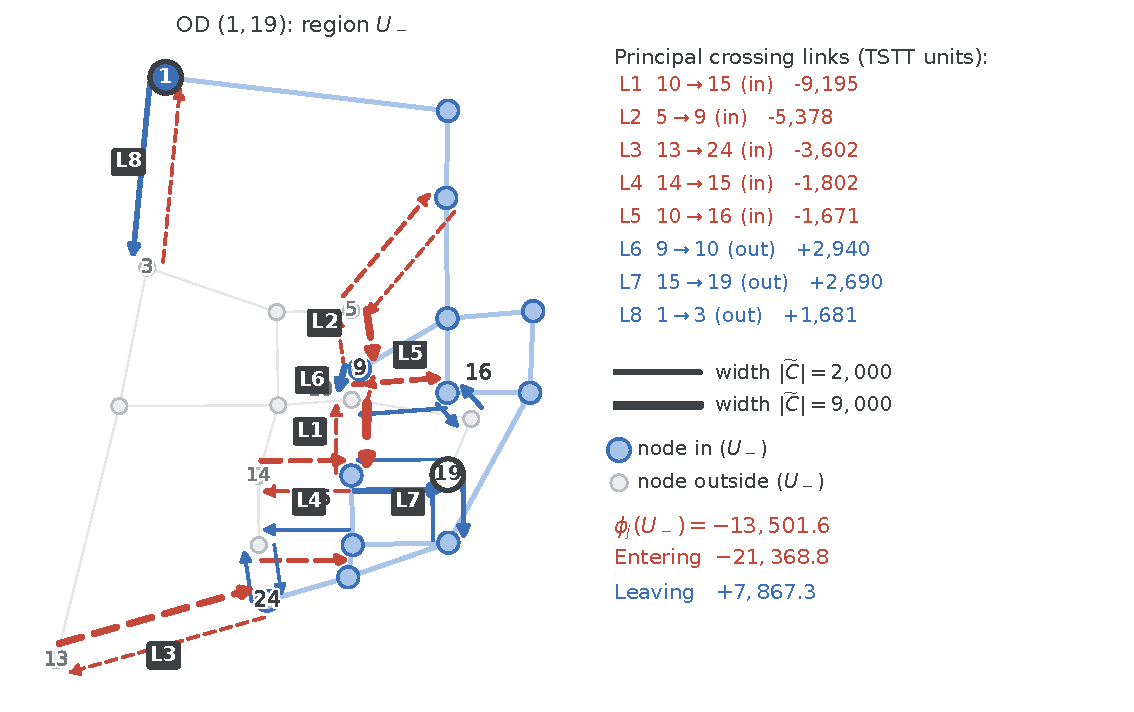
\includegraphics[width=0.95\linewidth]{../figures/fig_negmech_v102.pdf}
\caption{The connected minimizing region $U_-$ for OD $(1,19)$
(setting C, six-query protocol). Shaded nodes form $U_-$ (origin
node $1$ ringed; destination $19$ outside). Crossing-link arrows keep
the link direction; width scales with $|\widetilde C_{e,j}|$, and
colour and style encode the signed contribution to $\phi_j(U_-)$,
$a_{e,j}=\sigma_e\widetilde C_{e,j}$ ($\sigma_e=+1$ leaving, $-1$
entering; solid blue positive, dashed red negative), so a positive
attribution on an entering link appears red. The side panel lists, in
TSTT units, the five largest negative and three largest positive
contributions among the $26$ crossing links
($\mathrm{L}1$--$\mathrm{L}5$ negative, $\mathrm{L}6$--$\mathrm{L}8$
positive, ``(in)''/``(out)'' marking entering and leaving links),
with the width scale and the membership legend.}
\label{fig:negmech}
\end{figure}
\textbf{Endpoint identity checks.}
Appendix~\ref{supp:accuracy} reports the per-edge
endpoint-identity errors and their relation to completeness gaps on
these same demand paths.

\FloatBarrier
\subsection{Baseline surrogate envelopes}\label{supp:baselineenvelopes}
\begin{table}[pos=htbp]
\caption{Full-background surrogate validation on the identical
$41$-state path of the six-query protocol (setting C; TSTT units;
contributions and extrema rounded to integers, errors to one
decimal). $C_j^{\mathrm{learned}}$ and the connected extrema:
across-seed envelopes of per-model values (direct-SUE values in
Table~\ref{tab:newod}). Last two columns: five-seed
\emph{median} of the largest connected-boundary disagreement
$\epsilon_j^{\mathrm{cut}}$, in absolute units and as a percentage of
the direct connected span.}
\label{tab:fullbgsurrogate}
\small
\begin{tabular*}{\tblwidth}{@{\extracolsep{\fill}}lrrrrr}
\toprule
& & \multicolumn{2}{c}{Connected extrema: across-seed ranges}\\
\cmidrule(lr){3-4}
OD & $C_j$: across-seed envelope & per-model minima & per-model maxima & $\epsilon^{\mathrm{cut}}$ (med.) & $\epsilon^{\mathrm{cut}}$/span (med., \%)\\
\midrule
$(7,18)$ & $[574,\ 681]$ & $[335,\ 521]$ & $[907,\ 1{,}299]$ & $397.5$ & $522.5$ \\
$(1,19)$ & $[49{,}929,\ 51{,}452]$ & $[-13{,}911,\ -13{,}334]$ & $[23{,}683,\ 23{,}948]$ & $1{,}567.4$ & $4.2$ \\
$(4,5)$ & $[2{,}535,\ 2{,}934]$ & $[1{,}654,\ 2{,}148]$ & $[2{,}946,\ 3{,}546]$ & $1{,}050.8$ & $99.5$ \\
$(1,15)$ & $[77{,}416,\ 80{,}233]$ & $[-7{,}717,\ -6{,}766]$ & $[39{,}473,\ 40{,}076]$ & $2{,}187.3$ & $4.5$ \\
$(6,8)$ & $[73{,}565,\ 75{,}224]$ & $[36{,}412,\ 37{,}631]$ & $[66{,}892,\ 67{,}762]$ & $2{,}163.2$ & $6.9$ \\
$(7,12)$ & $[116{,}562,\ 118{,}706]$ & $[-17{,}084,\ -15{,}198]$ & $[59{,}965,\ 61{,}169]$ & $4{,}111.3$ & $5.3$ \\
\bottomrule
\end{tabular*}
\end{table}



\subsection{Fixed-screenline surrogate comparisons}\label{supp:screenlinelearned}
\begin{table}[pos=htbp]
\caption{Fixed straight screenlines: reference minimum and the five frozen flow-supervised surrogates at that same screenline (TSTT units). The last column gives the largest error over the screenline family, as an across-seed range.}
\label{tab:screenlinelearned}
\small\begin{tabular*}{\tblwidth}{@{\extracolsep{\fill}}lrrr}\toprule
OD & Reference minimum & Learned account: seed range & Maximum screenline error: seed range\\\midrule
$(7,18)$ & 642.4 & $[576.9,\ 789.8]$ & $[141.0,\ 269.4]$ \\
$(1,19)$ & -2766.6 & $[-3886.6,\ -3365.1]$ & $[857.9,\ 1430.8]$ \\
$(4,5)$ & 2652.3 & $[2301.7,\ 2918.8]$ & $[438.0,\ 648.3]$ \\
$(1,15)$ & 511.1 & $[732.8,\ 2068.2]$ & $[1140.6,\ 2553.0]$ \\
$(6,8)$ & 45230.2 & $[46431.5,\ 47218.3]$ & $[1276.2,\ 1988.1]$ \\
$(7,12)$ & -2967.3 & $[-2810.4,\ -1916.6]$ & $[1736.8,\ 2499.2]$ \\
\bottomrule\end{tabular*}\end{table}


\paragraph{Sign preservation.}\label{subsec:precision}
All five baseline seeds retain the three connected-family sign crossings
and positive system contributions. At the fixed reference extrema,
$m_j=\min\{-\phi_j^S(U_-),\phi_j^S(U_+)\}-\epsilon_j^{\rm conn}$
is positive, with smallest value 5519 TSTT units. This verifies sign
preservation without implying accurate column magnitudes.

At the fixed direct-model minimizing screenline, every baseline seed
retains the negative sign for both queries: $(1,19)$ gives
$[-3886.6,-3365.1]$ against the reference $-2766.6$, and $(7,12)$
gives $[-2810.4,-1916.6]$ against $-2967.3$. Their largest family-wide
errors across seeds are $1430.8$ and $2499.2$, below the respective
reference sign margins. These are screenline-specific certificates;
they supplement the separate connected-family result above
(Appendix~\ref{supp:screenlinelearned}).


The eight-query path-set and dispersion checks are collected in
Appendix~\ref{supp:coverage}. Boundary variation persists, although
the specified $(10,16)$ comparison $\{10\}\to\{10,17\}$ changes sign
across $\theta$; these are different fixed-path models, not convergence
to unrestricted SUE.

\subsection{Final learning comparison: budgets and groups}
Tables~\ref{tab:pair-budget-v102} and~\ref{tab:pair-groups-v102} report the fixed-budget and path-group breakdowns of the final comparison.
\begin{table}[t]\centering\small
\caption{Fixed-budget endpoint boundary error (\%) on six independent single-OD test paths. Seeds are averaged within each path before taking the path median.}
\label{tab:pair-budget-v102}
\begin{tabular}{lrrr}\toprule Method & 300 updates & 600 updates & 1,200 updates\\\midrule
Flow & 4.40 & 4.13 & 3.97\\
Flow + endpoint edge & 4.47 & 4.35 & 4.16\\
Flow + endpoint edge + cut & 4.51 & 4.38 & 4.17\\
Flow + response & 3.52 & 3.16 & 3.02\\
\bottomrule\end{tabular}\end{table}

\begin{table}[t]\centering\small
\caption{Mean unrestricted boundary error (\%) by number of active queries. Each group contains six independent paths, each balanced across queries.}
\label{tab:pair-groups-v102}
\begin{tabular}{lrrrr}\toprule Method & One OD & Two ODs & Three ODs & Six ODs\\\midrule
Flow & 14.34 & 18.24 & 19.71 & 19.80\\
Flow + endpoint edge & 11.11 & 15.72 & 16.06 & 18.93\\
Flow + endpoint edge + cut & 13.08 & 16.65 & 15.09 & 19.56\\
Flow + response & 12.67 & 16.30 & 13.45 & 13.73\\
\bottomrule\end{tabular}\end{table}


\subsection{Input-stratified OD coverage}\label{sec:coverage}
We select queries using only the published positive OD demand and directed free-flow shortest-path time. Each attribute is divided at its empirical tertiles, keeping ties in the lower group. In each of the nine cells, OD pairs are ordered lexicographically and the pairs at zero-based positions $\lfloor N/3\rfloor$ and $\lfloor2N/3\rfloor$ are retained. Empty cells remain empty and a singleton is retained once. This yields 18 queries from 528 positive demands. For each query, only its demand moves from $(1-a)q_j$ to $(1+a)q_j$, $a\in\{0.1,0.2\}$; all other demands remain at their published levels with endogenous route choice. Four endpoint equilibria per query give the exact single-OD edge attribution by Eq.~\eqref{eq:edgeidentity}, avoiding quadrature. The geometric family uses the same 36 pre-specified directions and connected-side filter as the screenline experiment.
\begin{table}[t]\centering\small
\caption{All input-stratified queries. Entries are geometric-account spreads for $\pm10\%$ and $\pm20\%$ intervals and their ratios to the exact unrestricted spread. Absolute values use the Sioux Falls cost units. No query is removed based on its attribution.}\label{tab:coverage}
\begin{tabular}{lrrrr}\toprule
OD & $S_{\rm geo}^{10}$ & $S_{\rm geo}^{20}$ & $S_{\rm geo}^{10}/S_{\rm all}^{10}$ & $S_{\rm geo}^{20}/S_{\rm all}^{20}$\\\midrule
(4,3) & 53.0 & 105.9 & 0.353 & 0.353\\
(12,3) & 4.8 & 9.5 & 0.417 & 0.417\\
(6,1) & 816.1 & 1632.1 & 0.651 & 0.651\\
(15,6) & 2009.1 & 4018.1 & 0.672 & 0.672\\
(6,21) & 1176.4 & 2352.8 & 0.668 & 0.668\\
(18,14) & 889.5 & 1778.9 & 0.511 & 0.511\\
(8,4) & 7235.2 & 14470.6 & 0.646 & 0.646\\
(19,8) & 3266.6 & 6533.2 & 0.374 & 0.374\\
(11,6) & 2434.9 & 4869.9 & 0.626 & 0.626\\
(16,2) & 4366.2 & 8732.3 & 0.545 & 0.545\\
(8,21) & 1730.7 & 3461.5 & 0.424 & 0.424\\
(14,8) & 3318.4 & 6636.8 & 0.495 & 0.495\\
(11,15) & 5054.3 & 10108.8 & 0.337 & 0.337\\
(17,9) & 6509.7 & 13037.1 & 0.696 & 0.695\\
(10,12) & 11713.3 & 23426.2 & 0.539 & 0.539\\
(13,10) & 14211.4 & 28426.4 & 0.667 & 0.667\\
(1,10) & 9336.8 & 18673.5 & 0.603 & 0.603\\
(10,1) & 9428.5 & 18856.8 & 0.606 & 0.606\\
\bottomrule\end{tabular}\end{table}
The median geometric-to-unrestricted spread ratios are 0.574 and 0.574 for the two widths. These results describe this fixed input-stratified sample; they are not a probability sample of all demand conditions. Endpoint differences identify total edge accounts, but do not identify the same-state study/background response decomposition. That decomposition is evaluated separately in the mechanism experiments.

\subsection{Supplementary pointwise-supervision comparisons}\label{app:legacy-learning}\label{app:learning-protocol}\label{app:calibration-protocol}
Two earlier comparisons use the same five full-background flow-trained
models, original data split and three-layer 128-unit tanh architecture
with 5,280 path logits. All continuation runs use 600 Adam updates,
learning rate $3\times10^{-5}$, flow batches of 32 and response batches
of eight, cycling six queries. Reference derivatives at 256 training
states use sampling seed 20261029; 64 additional derivative states are
reserved for validation. Flow scales are $0.01$ times edgewise training
root-mean-square flows; response and boundary scales are querywise
training root-mean-square column norms and $\mathcal K_j$ values,
respectively. All losses average squared normalized errors. Model
response derivatives are obtained by automatic differentiation.

The fixed-coefficient comparison sets both added loss coefficients to one,
uses shared seed-specific flow minibatches, and retains the final update
without selection. Four test paths, generated before training with seed
101029, have one, two, three and six active queries, mixed directions and
baselines in $[0.65,1.3]$ times published demands. Each has 41 quadrature
states. Attribution metrics summarize 60 active query--path--seed units,
flow metrics five seeds and increment metrics 20 path--seed pairs.
Boundary errors divide by $\mathcal K_j(\widetilde C^S_{:,j})$; column,
system and increment errors divide by the corresponding reference norm
or absolute value. These descriptive units are not treated as independent
paths for inferential statistics.
\begin{table}[t]
\centering\small
\caption{Equal-update continuation from five flow-trained checkpoints on four independent demand paths. Entries are medians over 60 active query--path--seed combinations, except flow (five seeds, held-out split) and increment error (20 path--seed pairs). Boundary error uses all separating cuts and is normalized by the corresponding maximum absolute reference account.}
\label{tab:structured-learning}
\begin{tabular}{lrrrrrr}\toprule
Method & Flow (\%) & Increment (\%) & Column (\%) & System (\%) & Cut abs. & Cut (\%)\\\midrule
Original & 0.04 & 5.18 & 14.11 & 2.08 & 260.55 & 9.93\\
Flow continuation & 0.03 & 5.34 & 12.29 & 1.48 & 268.81 & 9.98\\
Flow + response & 0.03 & 5.48 & 11.92 & 1.65 & 283.64 & 9.64\\
Flow + response + boundary & 0.12 & 14.07 & 32.01 & 1.97 & 708.35 & 22.25\\
\bottomrule\end{tabular}
\end{table}

Adding the boundary term increases pooled boundary error from 9.64\% to
22.25\%, although it improves 14/15 $(7,18)$ units and 8/10 $(4,5)$
units; the other query groups worsen. Reference labels and test paths
require 83.3\,s. Median continuation times are 105.6, 184.8 and 244.5\,s
for flow, response and boundary methods. Maximum conservation residual
is $4.6\times10^{-11}$; relative quadrature completeness discrepancy is
at most $5.1\times10^{-6}$.

The calibrated comparison selects $\lambda_{\rm cut}$ from
$\{0.001,0.01,0.1\}$ on seed zero, using the 64 reserved validation
states. It minimizes normalized boundary-response mean square subject
to validation flow error at most 110\% of the response comparator.
The chosen coefficient is then applied to all five seeds, reusing its
seed-zero fit: seven structural fits in total. Validation flow errors
are $0.0610\%$ for the response comparator and $0.0611\%$, $0.0631\%$,
$0.0804\%$ for the candidates; corresponding boundary-response mean
squares are $0.7040$, $0.6852$, $0.6097$, $0.4532$. Thus $0.1$ fails
the flow criterion and $0.01$ is selected. This additional search budget
precludes an equal-search advantage claim. Four new test paths use seed
101030 and the same active-query templates, with evaluation after
selection; the original paths remain diagnostic data.
\begin{table}[t]
\centering\small
\caption{Exploratory validation-calibrated continuation ($\lambda_{\mathrm{cut}}=0.01$), tested on four new independent demand paths (seed 101030). Entries are medians over 60 active query--path--seed combinations, except flow (five seeds, held-out split) and increment error (20 path--seed pairs). Boundary error uses all separating cuts and is normalized by the corresponding maximum absolute reference account.}
\label{tab:calibration-learning}
\begin{tabular}{lrrrrrr}\toprule
Method & Flow (\%) & Increment (\%) & Column (\%) & System (\%) & Cut abs. & Cut (\%)\\\midrule
Original & 0.04 & 5.40 & 12.22 & 1.65 & 289.36 & 7.47\\
Flow continuation & 0.03 & 5.12 & 11.45 & 1.32 & 261.00 & 7.44\\
Flow + response & 0.03 & 5.32 & 11.69 & 1.33 & 264.80 & 7.44\\
Calibrated boundary & 0.03 & 5.64 & 11.92 & 1.68 & 275.14 & 7.74\\
\bottomrule\end{tabular}
\end{table}

Calibration gives no overall improvement over response supervision:
new-path boundary error is 7.74\% versus 7.44\%, and column error
11.92\% versus 11.69\%. For $(4,5)$ all ten paired boundary errors
improve (group medians 48.65\% to 44.21\%); for $(7,18)$, eight of
fifteen improve but the group median rises from 85.70\% to 99.23\%.
On the original diagnostic paths, calibrated flow, increment, column,
system and boundary errors are $0.0342\%$, $5.35\%$, $12.56\%$,
$1.72\%$, and $324.11$ units ($10.09\%$). Candidate elapsed durations
sum to 829.4\,s (overlapping jobs, not CPU time); selected-fit median
time is 211.8\,s, new reference paths take 13.6\,s, and the complete
calibration/evaluation run takes 927.0\,s. New-path maximum conservation
residual and relative completeness discrepancy are $4.6\times10^{-11}$
and $9.2\times10^{-6}$. Complete paired results remain in the numerical
arrays. Neither supplementary comparison supports aggregate superiority
of boundary supervision.


\end{document}
